\section{Mathematical Model}

In this work, a two dimensional biological system is simulated with a mathematical model. The system is a culture dish of a monolayer of cells with virus diffusing over the cells. The model is a hybrid of an agent based model (ABM) and a partial differential equation model (PDEM) where the cells are represented with an ABM and the virus diffusion is represented by a PDEM.

\subsection{Viral transmission} \label{Viral_transmission}

When a virus is spreading among the cells in a culture dish, there is a probability that a healthy cell becomes infected by virus that is not within a cell, but flowing around and above the cell. When this viral transmission occurs it is called cell-free transmission. For cell-free transmission, the probability per unit time ($\mathrm{P_{cf}}$) that a cell becomes infected is determined by the amount of virus that is covering the cell ($V$) times the infection rate ($\beta$) \citep{holder11autoimm}, 
$$\mathrm{P_{cf}} = V \beta.$$ 
As a healthy cell becomes surrounded by more virus, the probability of cell-free infection increases. If the probability ($V \beta \Delta t$) is even greater than one due to the build up of virus, an adaptive time step is used. The time step ($\Delta t$) is divided in half repeatedly until the probability of cell-free infection is below one. Once the probability is finalized, a number from the uniform distribution is compared with the probability of cell-free infection. If that number is less than $\mathrm{P_{cf}}$, then the cell becomes infected.

%As the viral infection progresses, the total amount of virus in the culture dish changes. Plotting the amount of virus vs.\ time produces a curve that has a distinct shape and has characteristics that can be measured. The measurements, shown in Figure \ref{measurements}, can be used to compare multiple viruses or to compare multiple simulations of the same virus with different input parameters.

%\begin{itemize}
%\item \textbf{peak viral load:} The maximum amount of virus is commonly used as an indicator of the transmissibility of an infection \citep{handel09}. 
%\item \textbf{time of viral peak:} This is the time between the start of the infection and the peak of the virus and can give an indication of how quickly the virus is replicating.
%\item \textbf{viral upslope:} Viral upslope is the exponential growth rate of the viral titer before the peak is reached and is another indication of how quickly the virus is spreading from cell to cell. 
%\item \textbf{viral downslope:} \color{red}Text missing here.\color{black}
%\item \textbf{area under the curve (AUC):} AUC is often used to assess the severity of an infection \citep{hayden00, barroso05}.
%\item \textbf{infection duration:} The infection duration is indicative of how long an infected patient might test positive for presence of the virus. In this work $10^1 \mathrm{PFU/ml}$ is the threshold.
%\end{itemize}
%\begin{figure}
%\begin{center}
%    \resizebox{0.6\textwidth}{!}{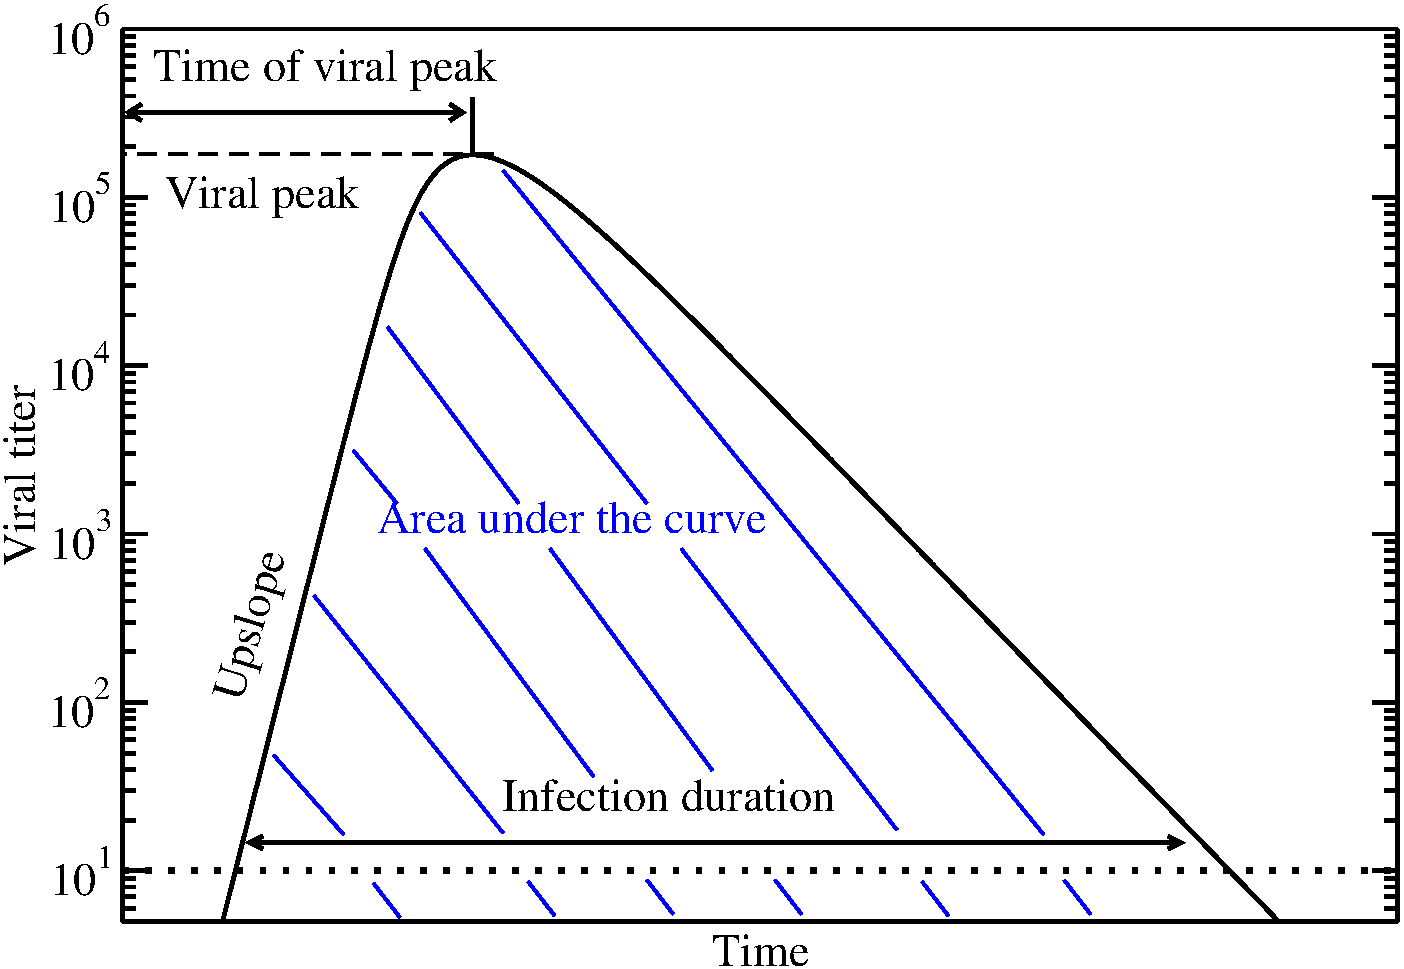
\includegraphics{Figures/measurements.pdf}}
%    \caption{Measurable characteristics of the viral titer curve.\color{red} Figure is missing downslope label.\color{black}}
%    \label{measurements}
%\end{center}
%\end{figure}

%1 - y = (1-m)^n

\subsection{Spatial accounting} \label{Spatial_accounting}

To allow for the two dimensional aspect of the culture dish to be represented in the model, the cells are approximated as hexagons. Using hexagons enables for an elegant managing of the cells' shapes in the dish and the viral transmission. Since the culture dishes are grown to confluence, the cells are close enough that they push on each other and the cell walls deform. This causes the cells to no longer be in the shape of a circle, but become irregular polygons with multiple sides \citep{bruckner_importance_2018}. Modeling the cells as hexagons gives the cells definite sides and the cells are able to span any two dimensional region forming a hexagonal grid. Furthermore, by using a hexagonal grid, when virus particles spread among this population of cells the indexing of the grid can be used to find the neighbors of any cell. This will be used for cell-free transmission to know where virus will flow away from (high concentrations areas) and to (low concentration areas) during diffusion. 

In addition to helping with the physical representation of the model, hexagonal coordinates have some other attributes that can be utilized to optimize the code for quicker compute times. The three attributes that this code utilizes are:
\begin{enumerate} 
    \item The coordinates can be split in to three sectors where the coordinates $X_{hex}$, $Y_{hex}$, and $Z_{hex}$ are simply cyclic permutations.
    \item The $X_{hex}$ and $Z_{hex}$ directions can be used as indices of a matrix.
    \item The coordinates of the neighboring hexagons are found by adding a cyclic permutation of 
        $\left [
            \begin{array}{c}
                1 \\
                0 \\
                -1\\
            \end{array}
        \right ]$
        for three of the neighbors and
        $\left [ 
            \begin{array}{c}
                1 \\
                -1 \\
                0\\
            \end{array}
        \right ]$
        for the other three neighbors.
\end{enumerate}
These attributes save time by either reducing the number of calculations needed or the amount of searching through data arrays. Attribute 1 allows for only a third of the cell locations to be calculated and Attributes 2 and 3 give the data a reference so that adjacent data in memory can be found quicker.

\subsection{Agent-based model} \label{ABM}

In an ABM, a system is broken down into smaller units called ``agents''. Each of the agents are governed by a set of rules on a local scale with large scale phenomena resulting from interaction of the agents, so the two scales are studied to find the connections. As a simulation of the model is stepped through time, the agents act and interact. These actions cause bulk properties, that may appear disconnected from the individual agents, to manifest. Properties are observed and measured to find the connection between the small interactions and large scale properties.

In this work, an ABM governs the transitions a cell makes through the stages of infection: healthy, eclipse, infected, and dead. A cell in the healthy state is an uninfected cell that remains healthy until infected. A cell in the eclipse state is an infected cell that is not yet producing virus. The cell remains in the eclipse state for an average amount of time, $\tau_E$. The specific time value for each cell is determined by a gamma distribution with shape value $\eta_E$ and scale value $\tau_E/\eta_E$. A cell in the infected state is an infected cell that is producing virus. The cell remains in the infected state for an average amount of time, $\tau_I$. The specific time value for each cell is determined by a gamma distribution with shape value $\eta_I$ and scale value $\tau_I/\eta_I$. A gamma (Erlang) distribution is used for the amount of time in the eclipse and infected phase, as suggested by the work of Beauchemin et al.\ \citep{beauchemin17} and Kakizoe et al.\ \citep{kakizoe15}. A cell in the dead state is a cell that can no longer change state, so once a cell is in the dead state the cell remains in that state until the end of the simulation. The flow of this is illustrated in figure \ref{fig:transitioning_through_the_stages_of_infection}.

The ABM uses four time arrays to track and transition the cells to different states after infection. The four arrays universal time (UT), healthy time (HT), eclipse time (ET), and infected time (IT) have an element for each cell. The universal time array holds the amount of time that each cell has been in the simulation; each element starts at zero and increases each iteration by the simulation's time step. The healthy time array holds the amount of time that a cell is healthy; each element starts at zero and while the cell is healthy increases each iteration by the simulation's time step. The eclipse time array holds the amount of time each cell is in the eclipse state and the infected time array holds the amount of time each cell is in the infected state. For the eclipse and infected arrays the amount of time is fixed and the value is determined by a gamma (Erlang) distribution, as described above. The flow of this is illustrated in figure \ref{fig:transitioning_through_the_stages_of_infection}.

%\begin{figure}
%    \centering
%    \begin{tikzpicture}[state/.style={regular polygon,regular polygon sides=6, draw, minimum size=2.5cm, inner sep=0pt, outer sep=0pt}]
%    \node[state, draw=AGreen, fill=AGreen!10] (H) {$Healthy$};
%    \node[state, draw=cyan, fill=cyan!10, right of=H] (E) {$Eclipse$};
%    \node[state, draw=red, fill=red!10, right of=E] (I) {$Infected$};
%    \node[state, draw=black, fill=black!10, accepting, right of=I] (D) {$Dead$};
%    
%    \draw   (H) edge[bend left=45] node [above] {} (E);
%    \draw   (E) edge[bend left=45] node [above] {$\tau_E$} (I);
%    \draw   (I) edge[bend left=45] node [above] {$\tau_I$} (D);
%    \end{tikzpicture}
%    \caption{The stages of infection healthy, eclipse, infected, and dead are shown. Cells stay in  the eclipse stage for an average time $\tau_E$ and in the infected stage for an average time $\tau_I$.}
%    \label{fig:stages_of_infection}
%\end{figure}

%\begin{figure}
%    \centering
%    \begin{tikzpicture}[state/.style={regular polygon,regular polygon sides=6, draw, minimum size=2.5cm, inner sep=0pt, outer sep=0pt}]
%        \node[state, draw=AGreen, fill=AGreen!10] (H) {$Healthy$};
%        \node[state, draw=cyan, fill=cyan!10, below right of=H] (E) {$Eclipse$};
%        \node[state, draw=red, fill=red!10, below right of=E] (I) {$Infected$};
%        \node[state, draw=black, fill=black!10, accepting, below right of=I] (D) {$Dead$};
%            
%        \draw   (H) edge[bend left=45] node [above right] {Infection event} (E);
%        \draw   (E) edge[bend left=45] node [above right] {UT $>$ HT + ET} (I);
%        \draw   (I) edge[bend left=45] node [above right] {UT $>$ HT + ET + IT} (D);
%    \end{tikzpicture}
%    \caption{Transitioning through the stages of infection: UT is the universal time for a cell, HT is the healthy time for a cell, ET is the eclipse time for a cell, and IT is the infected time for a cell.}
%    \label{fig:transitioning_through_the_stages_of_infection}
%\end{figure}

\begin{figure}
    \centering
    \begin{tikzpicture}[
        Healthy/.style={regular polygon,regular polygon sides=6, draw, minimum size=2.5cm, inner sep=0pt, outer sep=0pt, draw=AGreen, fill=AGreen!10},
        Eclipse/.style={regular polygon,regular polygon sides=6, draw, minimum size=2.5cm, inner sep=0pt, outer sep=0pt, draw=cyan, fill=cyan!10},
        Infected/.style={regular polygon,regular polygon sides=6, draw, minimum size=2.5cm, inner sep=0pt, outer sep=0pt, draw=red, fill=red!10},
        Dead/.style={regular polygon,regular polygon sides=6, draw, minimum size=2.5cm, inner sep=0pt, outer sep=0pt, draw=black, fill=black!10}]

        \node[Healthy] (H) {$Healthy$};
        \node[Eclipse, below right of=H] (E) {$Eclipse$};
        \node[Infected, below right of=E] (I) {$Infected$};
        \node[Dead, accepting, below right of=I] (D) {$Dead$};
            
        \draw   (H) edge[bend left=45] node [above right] {Infection event} (E);
        \draw   (E) edge[bend left=45] node [above right] {UT $>$ HT + ET} (I);
        \draw   (I) edge[bend left=45] node [above right] {UT $>$ HT + ET + IT} (D);

        \draw   (H) edge[bend right=45] node [below left] {} (E);
        \draw   (E) edge[bend right=45] node [below left] {$\tau_E$} (I);
        \draw   (I) edge[bend right=45] node [below left] {$\tau_I$} (D);

        %Legand with text
        \matrix [draw,
                below right,
                column 1/.style={anchor=base west},
                column 2/.style={anchor=base west}
                ] at (current bounding box.north east) 
        {
          \node [] {UT}; & \node [] {Universal time}; \\ 
          \node [] {HT}; & \node [] {Healthy time}; \\ 
          \node [] {ET}; & \node [] {Eclipse time}; \\ 
          \node [] {IT}; & \node [] {Infected time}; \\ 
        };

%        %Legand with nodes
%        \matrix [draw, below left] at (current bounding box.north east) {
%          \node [Healthy, scale=0.3, label=right:Healthy] {}; \\
%          \node [Eclipse, scale=0.3, label=right:Eclipse] {}; \\
%          \node [Infected, scale=0.3, label=right:Infected] {}; \\
%          \node [Dead, scale=0.3, label=right:Dead] {}; \\
%        };
    \end{tikzpicture}
\caption{The stages of infection: healthy, eclipse, infected, and dead are shown. The cells transition through the stages at different time points. Above: The time point when a state transition occurs is shown in terms of UT, the universal time, for a cell. %UT is the time a cell has existed, HT is the time a cell has been healthy, ET is the time a cell is in the eclipse phase, and IT is the time a cell is in the  infected.
Below: The time point when a state transition occurs is shown in terms of average time. $\tau_E$ is the average time a cell stays in  the eclipse stage and $\tau_I$ is the average time a cell stays in the infected stage. \label{fig:transitioning_through_the_stages_of_infection}}
\end{figure}

\subsection{Partial differential equation model} \label{PDEM}

PDEMs are used to model multiple dimensions; in this work a PDE in hexagonal coordinates is used to model the two-dimensional spatial spread of virus over cells in a culture dish. In a PDEM, the dynamics of a system can be represented by a partial differential equation, or more specifically, an equation that contains multi-variable functions that represent important system aspects and one or more partial derivatives of those functions. In the culture dish, as an infected cell releases virus into the extracellular fluid, the virus diffuses across a density gradient. The PDEM represents this diffusion with the diffusion equation, 
\begin{equation}
\frac{\partial V}{\partial t}=D \nabla^{2}V + p - cV, \label{diff_eq}
\end{equation}
where $V$ is the density of the virus, $D$ the diffusion coefficient, $p$ is the production rate per cell, $c$ is the viral clearance rate. In the code, along with the assumption of hexagonal cells, the cells are assumed to be flat, so the virus is diffusing over a smooth two dimensional plane. This assumption allows for the use of the two dimensional diffusion equation in hexagonal coordinates, so Eq.\ \eqref{diff_eq} becomes 
$$\frac{\partial V}{\partial t} = D\frac{2}{3} \left (\frac{\partial^2}{\partial x^2_1}+\frac{\partial^2}{\partial x^2_2}+\frac{\partial^2}{\partial x^2_3}\right )V + p -cV$$ 
where  
$\textbf{x}_1=
\left [
    \begin{array}{c}
        1 \\
        0 \\
    \end{array}
\right ]$, 
$\textbf{x}_2=
\left [
    \begin{array}{c}
        -1/2 \\
        \sqrt{3}/2 \\
    \end{array}
\right ]$, and 
$\textbf{x}_3=
\left [
    \begin{array}{c}
        -1/2 \\
        -\sqrt{3}/2 \\
    \end{array}
\right ]$ 
are the unit vectors for a hexagonal grid. For computation, we use a forward Euler implementation of the PDEM with Neumann boundary conditions.

\subsection{Parameters of viral spread}

The eight parameters $\beta$, $\tau_E$, $\eta_E$, $\tau_I$, $\eta_I$, $p$, $c$, and $D$ affect the dynamics of virus spread in the model. Four of the parameters, $\tau_E$, $\eta_E$, $\tau_I$, and $\eta_I$, are used in the ABM to choose the time duration that a cell is in the eclipse and infected phase as mentioned in section \ref{ABM}. Three of the other parameters, $p$, $c$, and $D$, are used in the PDEM and characterize the differential equation, as mentioned in section \ref{PDEM}. The final parameter, $\beta$, governs the interaction between the virus and cells, setting the probability that the cell is infected. In order to model a particular virus, values for these parameters need to be chosen. The initial values of the parameters are chosen from ordinary differential equation models of influenza and listed in Table \ref{tab_params} (viral titer units have been converted to virions, as described in \citep{dobrovolny17}). %For $\eta_E$, $\eta_I$, $c$, and $D$ the values are fixed, but for $\beta$, $\tau_E$, $\tau_I$, and $p$ the values serve as a starting point for the model to be fit to real experimental data.

\begin{table}
%\centering
\caption{Parameter values to simulate an influenza infection with the ABM/PDEM model.\label{tab_params}}
\resizebox{\textwidth}{!}{%
\begin{tabular}{llcr}
\hline
Parameter & Meaning & Value & Reference\\
\hline
$\beta$ & Infection rate & 2.0 $/\mathrm{h}$ & Scaled from Beauchemin et al.\ \citep{beauchemin08}\\
$p$ & Viral production rate & 562800 $/\mathrm{h}$ & Scaled from Beauchemin et al.\ \citep{beauchemin08}\\
$c$ & Viral clearance rate & 0.105 $/\mathrm{h}$ & Beauchemin et al.\ \citep{beauchemin08}\\
$D$ & Diffusion coefficient & 2.16$\times 10^{-8}$ $\mathrm{m}^2/\mathrm{h}$ & Stokes-Einstein equation\\
$\tau_E$ & Mean eclipse duration & 6.0 $\mathrm{h}$ & Beauchemin et al.\ \citep{beauchemin08}\\
$\eta_E$ & Eclipse shape parameter & 30 & Pinilla et al.\ \citep{pinilla12}\\
$\tau_I$ & Mean infectious lifespan & 12.0 $\mathrm{h}$ & Beauchemin et al.\ \citep{beauchemin08}\\
$\eta_I$ & Infectious shape parameter & 100 & Pinilla et al.\ \citep{pinilla12}\\
\end{tabular}}
\end{table}

%In order to determine which parameter values minimize the SSR, a brute force walk of a parameter space is performed. The axes of the parameter space are four arrays that are constructed around the initial values of $\beta$, $p$, $\tau_I$, and $\tau_E$, shown in Table \ref{tab_params}. Two values, increasing or decreasing by 25\%, are added on both sides of the initial points; resulting in a total of 5 points per array and 625 points total in the parameter space.

\subsection{Implementation on GPUs}

As the model becomes more complex, GPU acceleration via parallel programming is used to decrease the simulation run times and therefore increase the number of studies that can be conducted in a given time. In the simulations, the cells change state based on the amount of virus above them. The number of cells in a culture dish is on the order of $10^6$ cells \citep{Number_of_cells_in_a_dish_noauthor_useful_nodate}, so the ABM will simulate a grid of $1001365$ agents of hexagonal cells in a circle to best replicate what is happening in the experiment. Each agent will follow the rules of checking the amount of virus above the cell every time step. Utilizing attribute 2 of hexagonal coordinates, the number of calculations is reduced from the order of ($\mathcal{O}(n^2)$) per time step to the order of the number of agents ($\mathcal{O}(n)$). The calculations from the agents' rules are split over the processing units of a GPU to be calculated in parallel or simultaneously. To utilize this processing, Nvidia's CUDA (Compute Unified Device Architecture) is used to implement the ABM and PDEM. CUDA is an Application Programming Interface (API) that allows the many processing units (cores) on a Nvidia brand GPU to be used for computing. %The ability to manipulate what is happening at the cellular level of the simulations allows for generation of isolated studies of the viral transmission. The isolated studies of how cells are infected are analyzed and the characteristics from section \ref{Viral_transmission} are compare to find any trends in the data



%%%%%%%%%%%%%%%%%%%%%%%%%%%%%%%%%%%%%%%%%%%%%%%%%%%%%%%%%%%%%%%%%%%%%%%%%%%%%%%%%%
\subsection{Convergence Testing}

Partial differential equations (PDEs) are a popular way to model systems that evolve over both space and time, an example is discussed in section \ref{PDEM}. With PDEs, even systems that have an exact solution need to be calculate on a computer, because of the infinite series that are required in those solutions. So solutions to PDEs are often found through numerical integration. In the numerical integration, space and time are assumed to be made up of small units (discretization). Time is a one dimensional line of points separated by a chunk of time called $\Delta t$ and space is a grid with a line of points for each dimension where there is a chunk of space for each dimension $\Delta x$, $\Delta y$ (two dimensional Cartesian space). At these points in time and space, a numerical integration scheme (numerical scheme) for approximating the solution of the PDE is chosen. Different numerical schemes have different benefits. Depending on the phenomena that needs to be studied with the PDE the size of $\Delta t$, $\Delta x$, and $\Delta y$ and the choice of numerical scheme are important. If the chunks of space or time are too large then the simulation does not have the resolution to resolve phenomena that occur at smaller increments in the model and if the numerical scheme requires to much computing power then the solutions can not be found in a timely manner.

From the choice of numerical scheme a conditional relationship between $\Delta t$, $\Delta x$, and $\Delta y$ is formed and must be met. For the Euler's method $$ \frac{\Delta t}{(\Delta x)^{2}} \leq \frac{1}{2},$$ if we make $\Delta x = \Delta y$.\citep{} This relationship is necessary to ensure that the sequence of approximations, that the numerical scheme uses to approximate a solution, converges and not allow the error to grow exponentially to a point that the solutions are unreliable. Using the relationship above, a value for $\Delta t$, $\Delta x$, and $\Delta y$ can be chosen to ensure stability of the error in the numerical scheme. As long as that relationship is met the solution is reliable within a certain error, but the relationship does not give the $\Delta t$, $\Delta x$, and $\Delta y$ that are best for producing accurate simulations with the least amount of computing cost.

To ensure the simulation of the PDEM converges, we need to optimize the space and time discretizations: $\Delta t$, $\Delta x$, and $\Delta y$. Convergence testing is a simple brute force method where the input parameters are increased or decreased by a particular amount and the accuracy or trends of the simulation are measured for each of the the new increments. Schemes for convergence testing are implemented and studied in fields like computational fluid dynamics \citep{bermejo16,kim20fluid} and astrophysics \citep{xu21,banei21}. The model proposed in this work has fixed $\Delta x$ and $\Delta y$, because the simulations are of real cells, whose average diameter can be measured between \numrange[range-phrase = --]{50}{100}\si{\micro\meter}. Thus the convergence testing only has to be conducted for $\Delta t$. To conduct the study a starting point of 0.005 hr was chosen and a range of seven values was created by multiplying or dividing the initial $\Delta t$ by 2 repeatedly. For each of these $\Delta t$s, the median viral titer curve of ten simulations were compared.

\subsection{Data Fitting} \label{Data_Fitting}

As part of our model validation, we verified that the model could reproduce viral titer curves observed experimentally. The experimental data set used here is from an \emph{in vitro} experiment performed by Pinilla et al.\ \citep{pinilla12}. During the study, a well of a 24-well plate, containing Madin-Darby canine kidney (MDCK$\alpha$2,6) cells was inoculated with the A/Qu\'{e}bec/144147/09 (H1N1) pandemic strain of influenza virus and the supernatant fluid was collected every 6 hours until 36 hours and then every 12 hours until 72 hours post infection. The supernatant was then used for RNA isolation and/or viral titration by standard plaque assay on MDCK$\alpha$2,6 cells. The specific data referenced for this work is the multiple-cycle viral yield experiment shown in figure 2A of the Pinilla manuscript.

To determine the best fit of the model to the experimental data, the sum of square residuals (SSR) is minimized, $$\mathrm{SSR} = \sum_{i=1}^{n} (y_i - \hat y_i)^{2},$$ where $y_i$ is from the experimental data set and $\hat y_i$ is from the simulated data set. In our case, the simulated data set is the average of ten cell-free transmission simulations. The initial conditions for the simulations are: Total cells -- $1001365$, Total virus -- $0.0$, and MOI -- $5\times 10^{-5}$. To perform the minimization, a separate code that utilizes the function \texttt{minimize} from the python package \texttt{scipy}, was written. In the code, five parameters ($\beta$, $p$, $\tau_I$, $\tau_E$, and $c$) are allowed to vary and the remaining parameters are held fixed to the values given in Table \ref{tab_params}. The minimization code is given an initial guess for the five parameters, then by the Nelder-Mead method the next set of parameters is produced, until the minimum SSR is found.
%%%%%%%%%%%%%%%%%%%%%%%%%%%%%%%%%%%%%%%%%%%%%%%%%%%%%%%%%%%%%%%%%%%%%%%%%%%%%%%%%%%
\section{Results}

\subsection{Model simulation}

Using the influenza parameters of Table \ref{tab_params}, we simulated an infection initiated with 1001365 cells in a dish, an MOI of $10^{-4}$, and no initial virus. Figure \ref{fig_FullDish_cellandvirus} shows different views of plaques forming in the entire dish. On the left are cells in the different stages of infection described in section \ref{ABM}, where the healthy cells are colored green, eclipse cells are colored cyan, infected cells are colored red, and dead cells are colored black. On the right are figures showing the corresponding virus concentrations that are over the cells, where areas of higher concentration are colored yellow and areas of lower concentration are colored purple. Figure \ref{fig_FullDish_cellandvirus} shows the infection in 5 hour increments starting at 5 hours, when no cells are producing virus, and ending at 60 hours, when almost all the cells have died. The ABM reproduces the plaques typically seen in experimental \emph{in vitro} infections \citep{holder11H274Y}. 

For a closer look at the plaques, figure \ref{fig_ZoominDish} is a zoomed in view of the infection at hours 6.5, 11.5, and 16.5. The cells are shown on the left, with the same color scheme used in figure \ref{fig_FullDish_cellandvirus}, and the corresponding virus distribution is shown on the right. Here we can clearly see the heterogeneous growth of the plaque; it is not simply a radially symmetric change of cells from eclipse to infectious. 

\begin{figure}
\centering
\begin{minipage}{0.8\linewidth}
\centering
\begin{multicols}{2}
    \resizebox{0.48\textwidth}{!}{%
        
\includegraphics[width=0.48\textwidth]{Figures/Full-Dish-CellPhotos/cell9.png}
        
\includegraphics[width=0.48\textwidth]{Figures/Full-Dish-VirusPhotos/virus9.png}}

    \resizebox{0.48\textwidth}{!}{%
        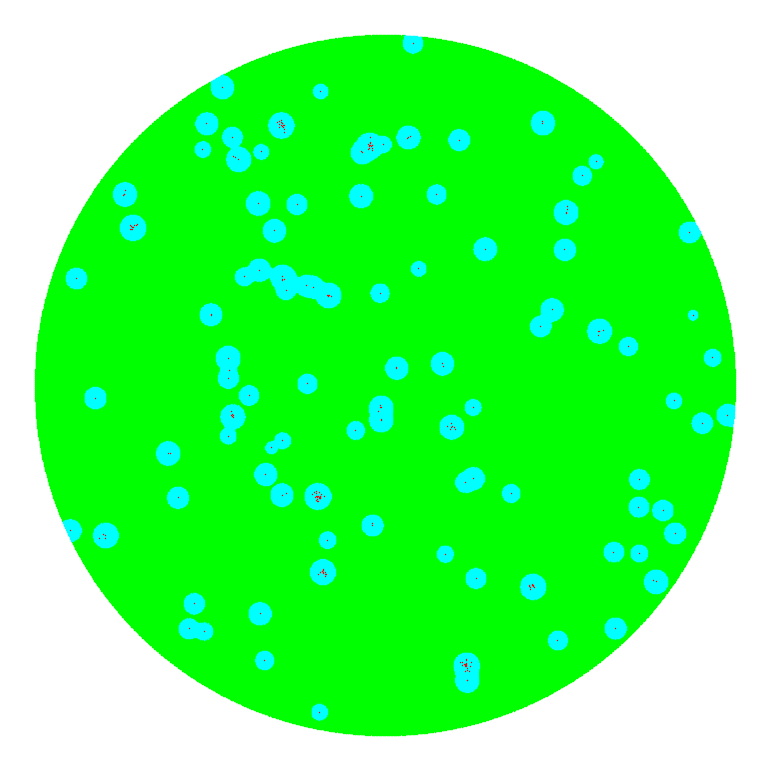
\includegraphics[width=0.48\textwidth]{Figures/Full-Dish-CellPhotos/cell19.png}
        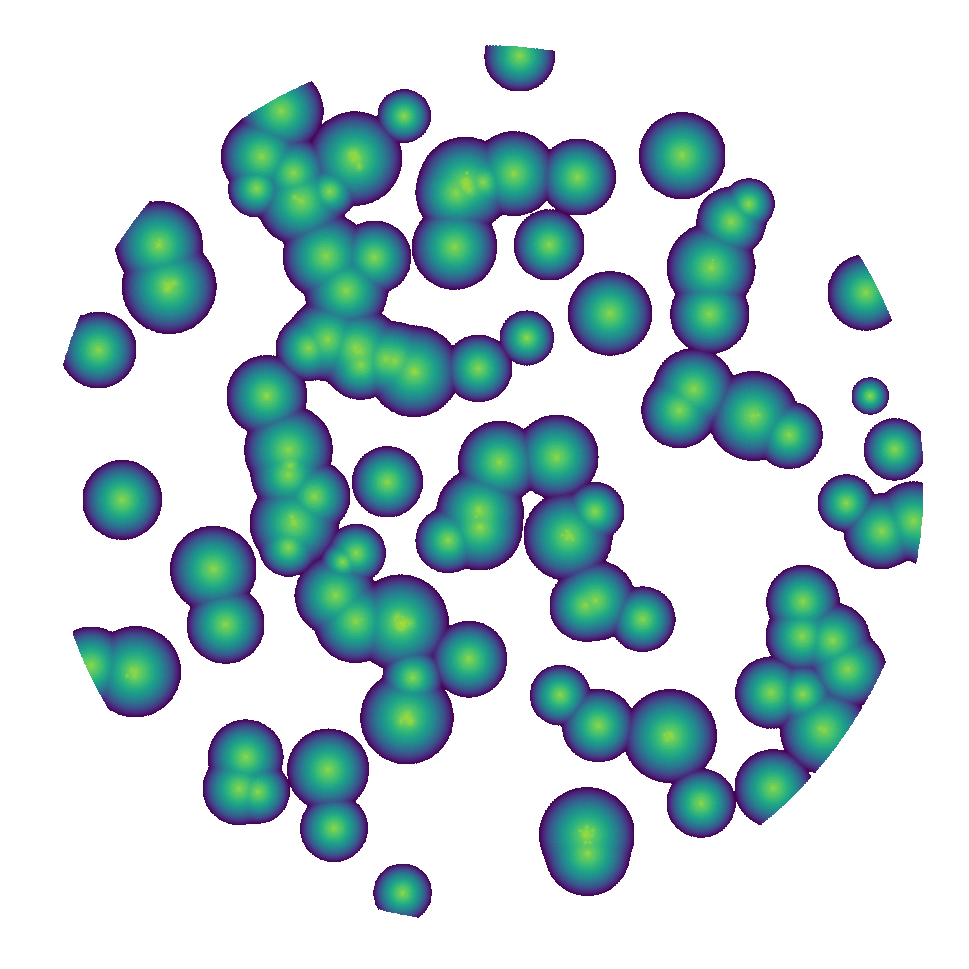
\includegraphics[width=0.48\textwidth]{Figures/Full-Dish-VirusPhotos/virus19.png}}

    \resizebox{0.48\textwidth}{!}{%
        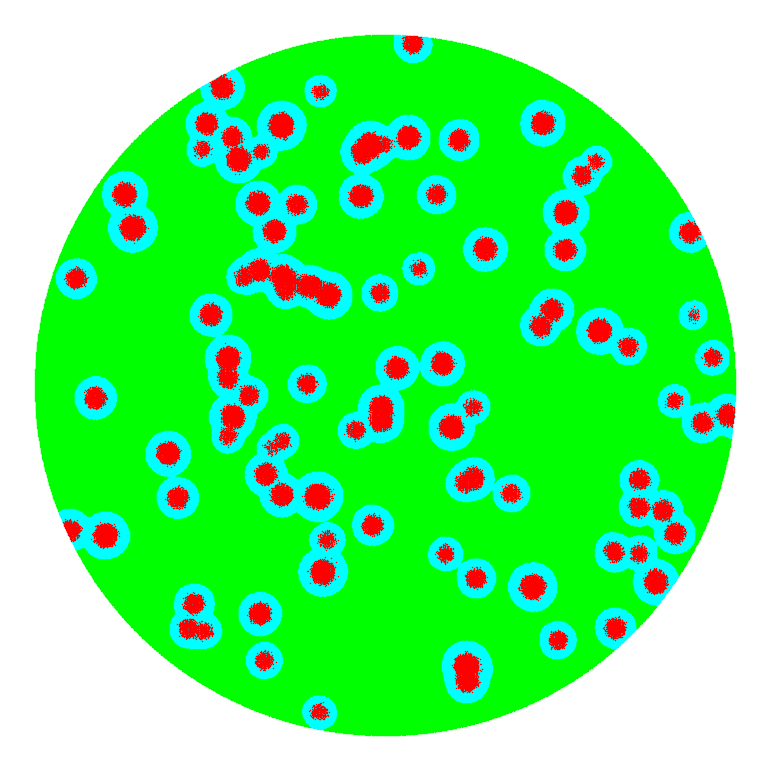
\includegraphics[width=0.48\textwidth]{Figures/Full-Dish-CellPhotos/cell29.png}
        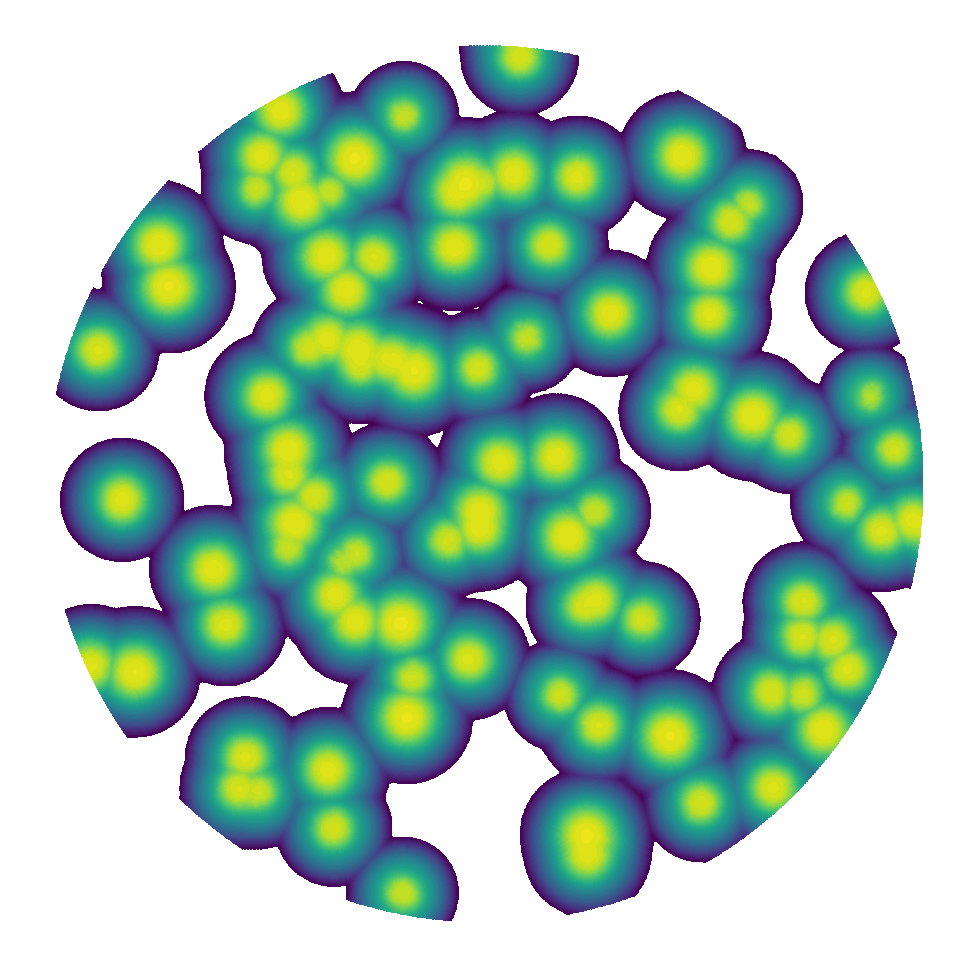
\includegraphics[width=0.48\textwidth]{Figures/Full-Dish-VirusPhotos/virus29.png}}

    \resizebox{0.48\textwidth}{!}{%
        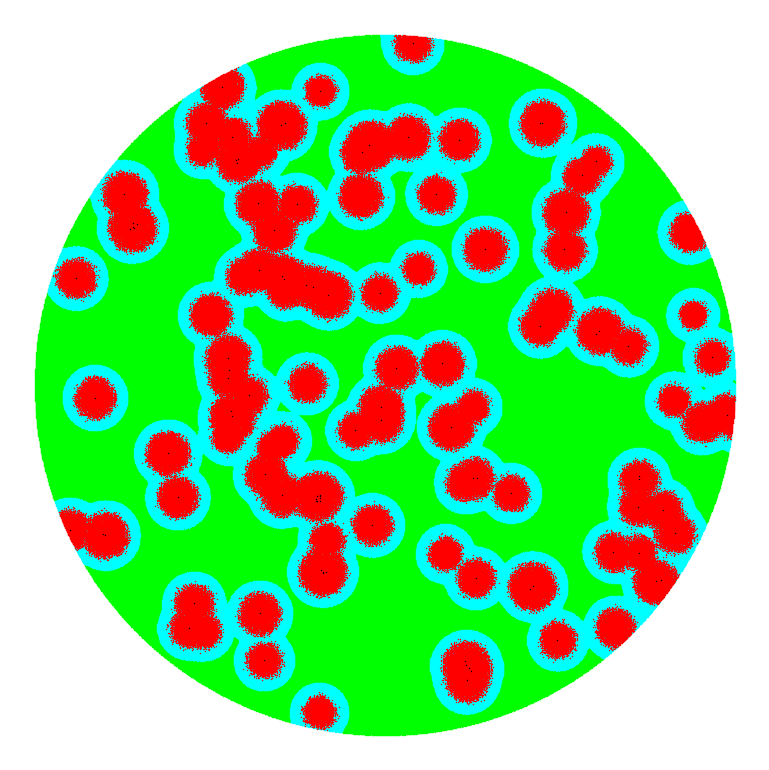
\includegraphics[width=0.48\textwidth]{Figures/Full-Dish-CellPhotos/cell39.png}
        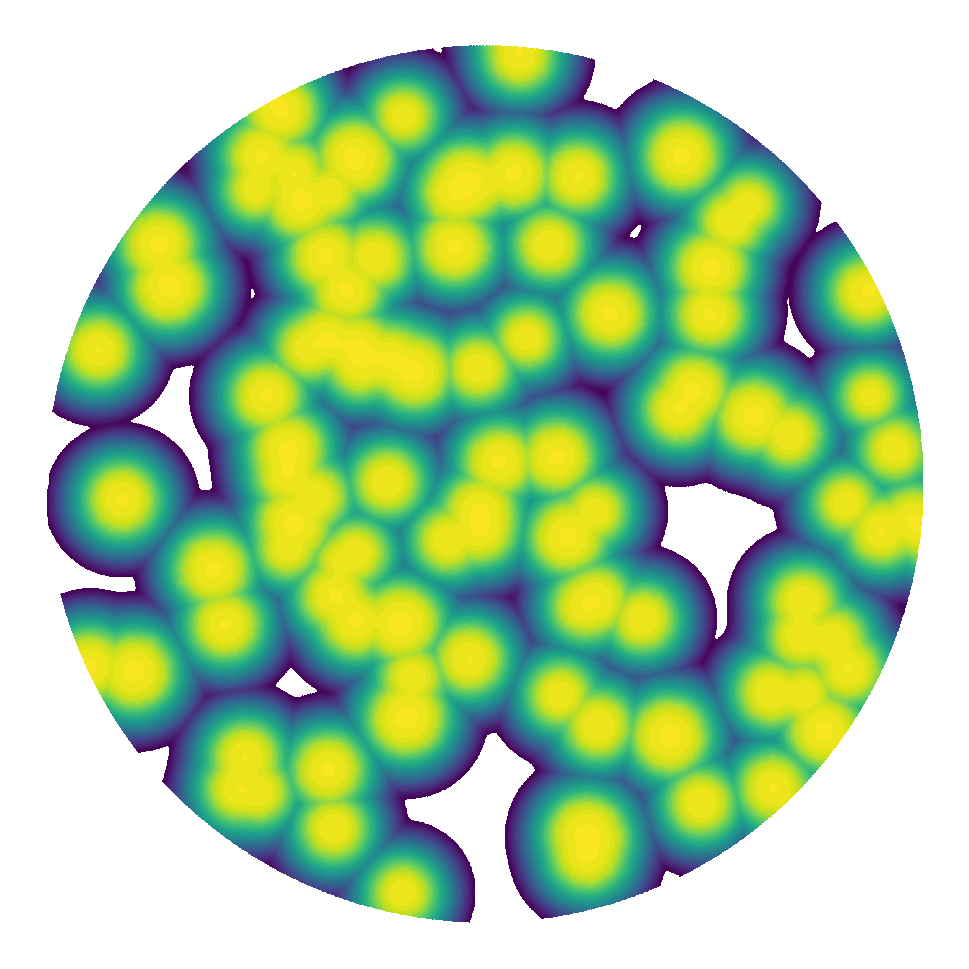
\includegraphics[width=0.48\textwidth]{Figures/Full-Dish-VirusPhotos/virus39.png}}

    \resizebox{0.48\textwidth}{!}{%
        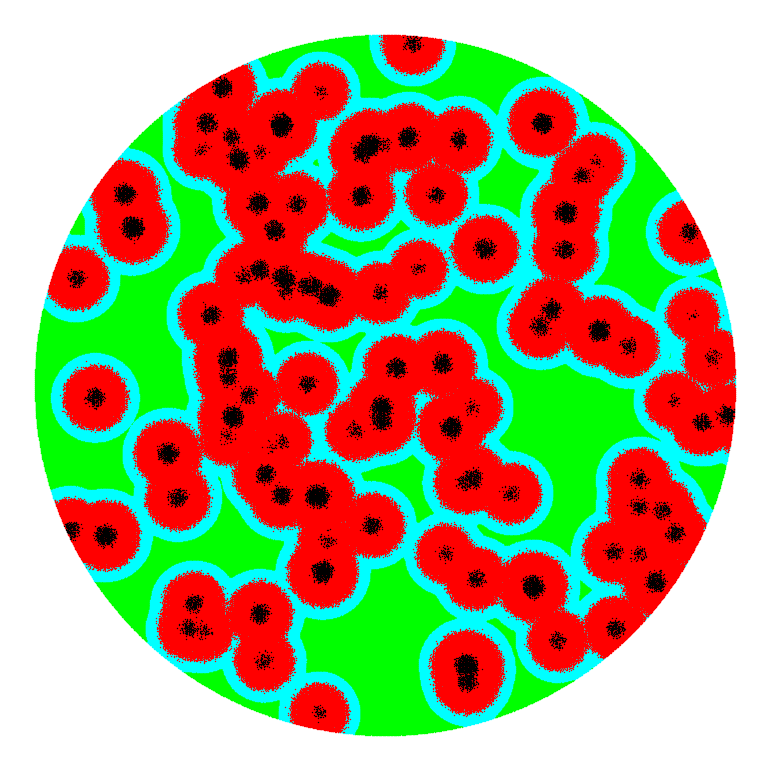
\includegraphics[width=0.48\textwidth]{Figures/Full-Dish-CellPhotos/cell49.png}
        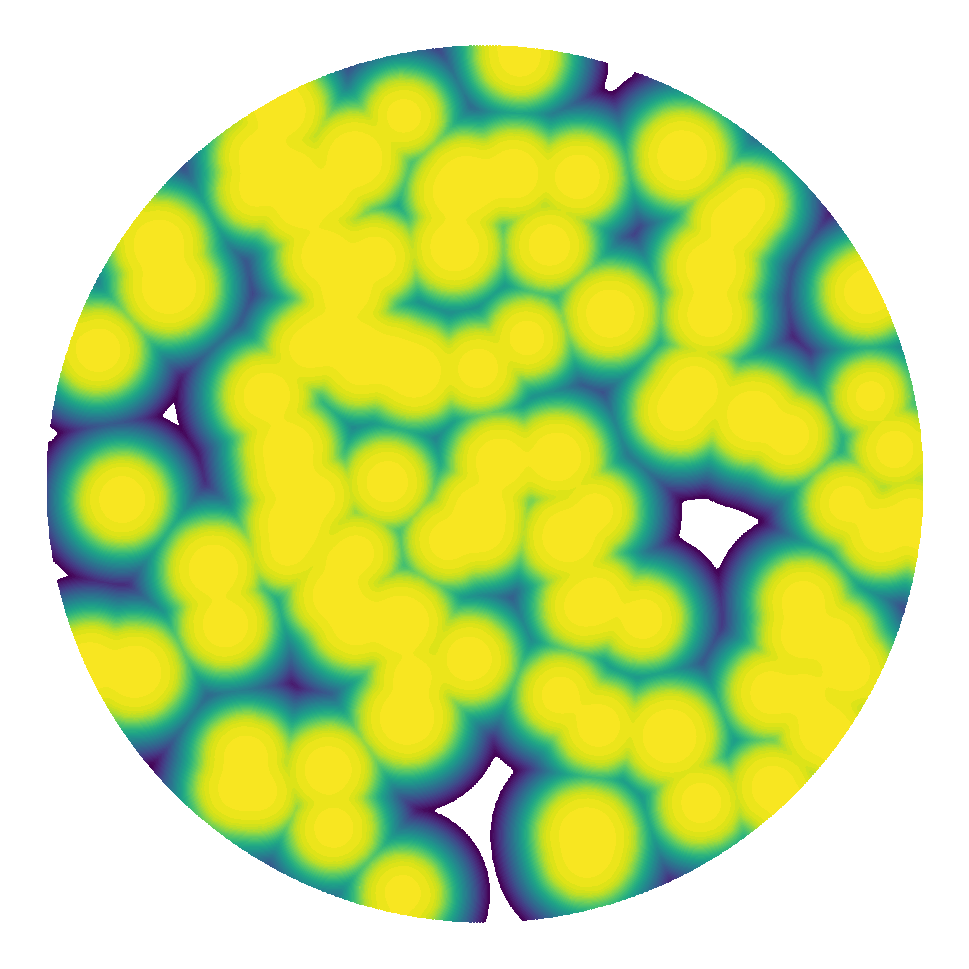
\includegraphics[width=0.48\textwidth]{Figures/Full-Dish-VirusPhotos/virus49.png}}

    \resizebox{0.48\textwidth}{!}{%
        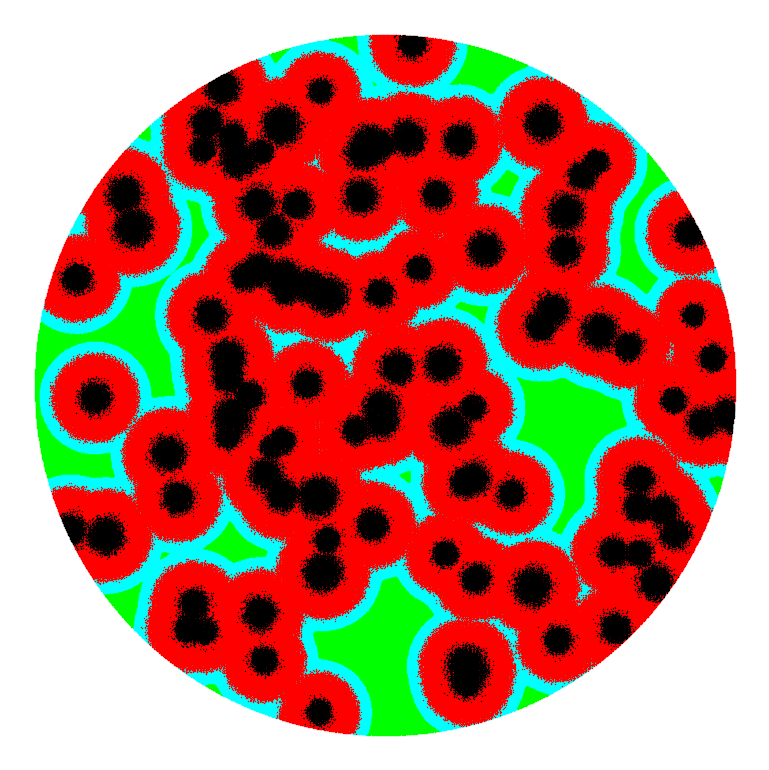
\includegraphics[width=0.48\textwidth]{Figures/Full-Dish-CellPhotos/cell59.png}
        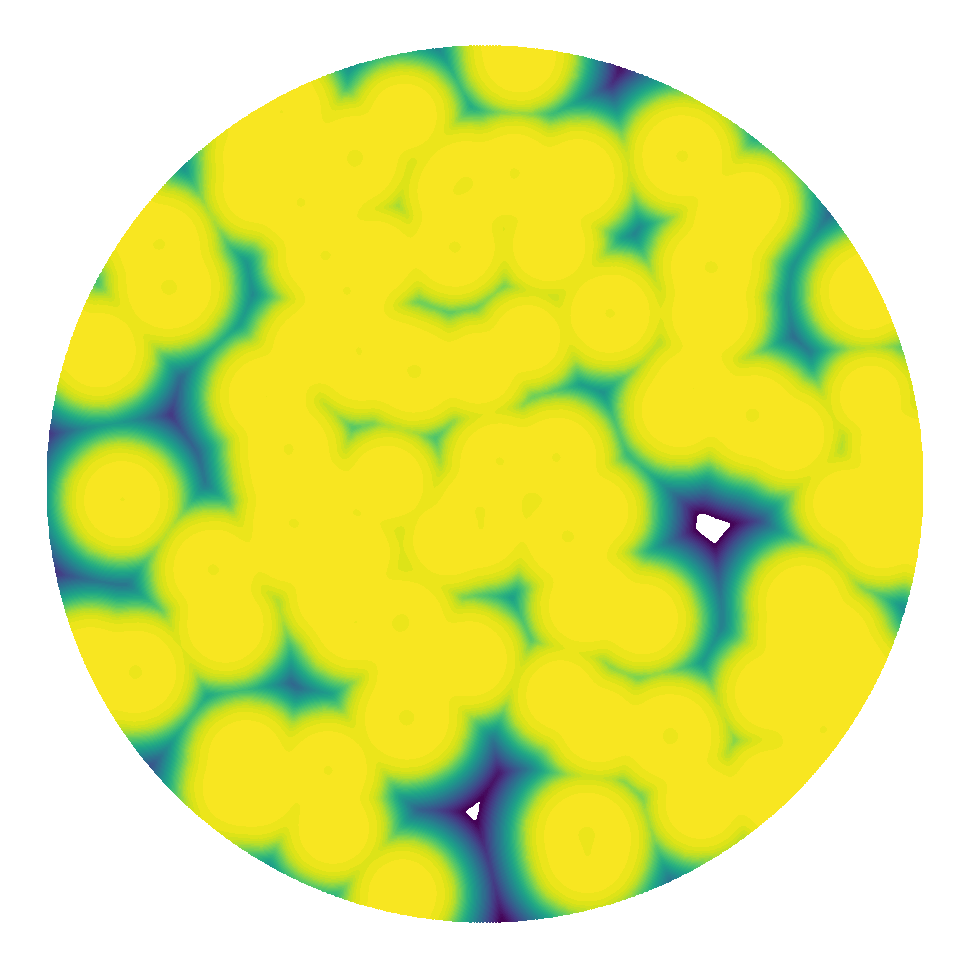
\includegraphics[width=0.48\textwidth]{Figures/Full-Dish-VirusPhotos/virus59.png}}

    \resizebox{0.48\textwidth}{!}{%
        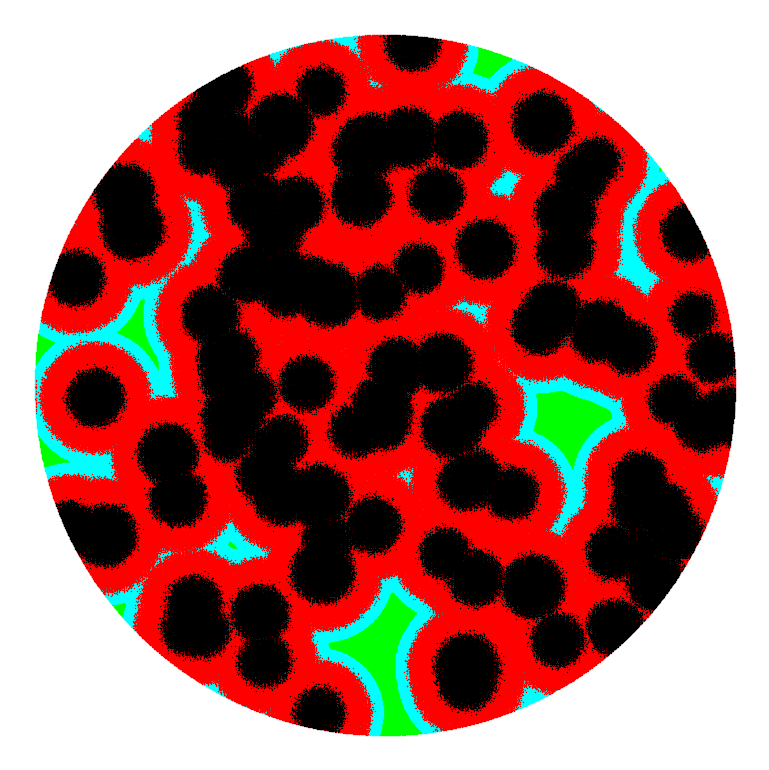
\includegraphics[width=0.48\textwidth]{Figures/Full-Dish-CellPhotos/cell69.png}
        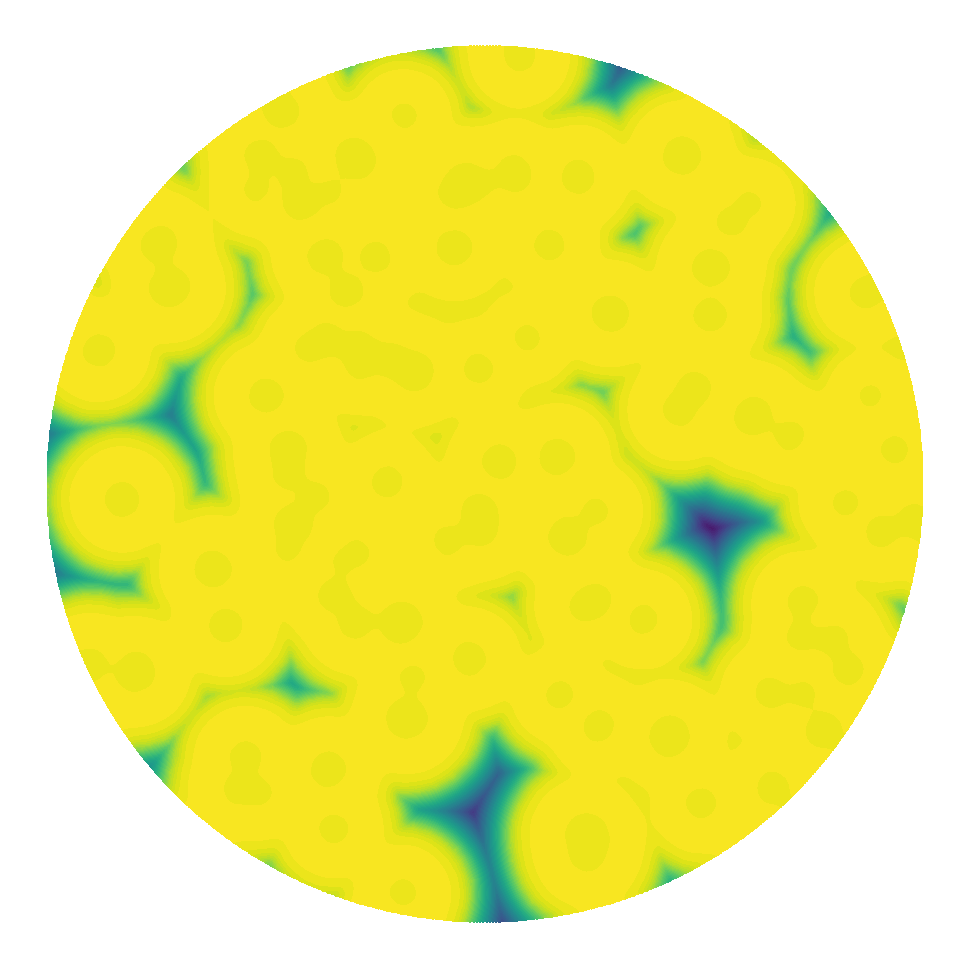
\includegraphics[width=0.48\textwidth]{Figures/Full-Dish-VirusPhotos/virus69.png}}

    \resizebox{0.48\textwidth}{!}{%
        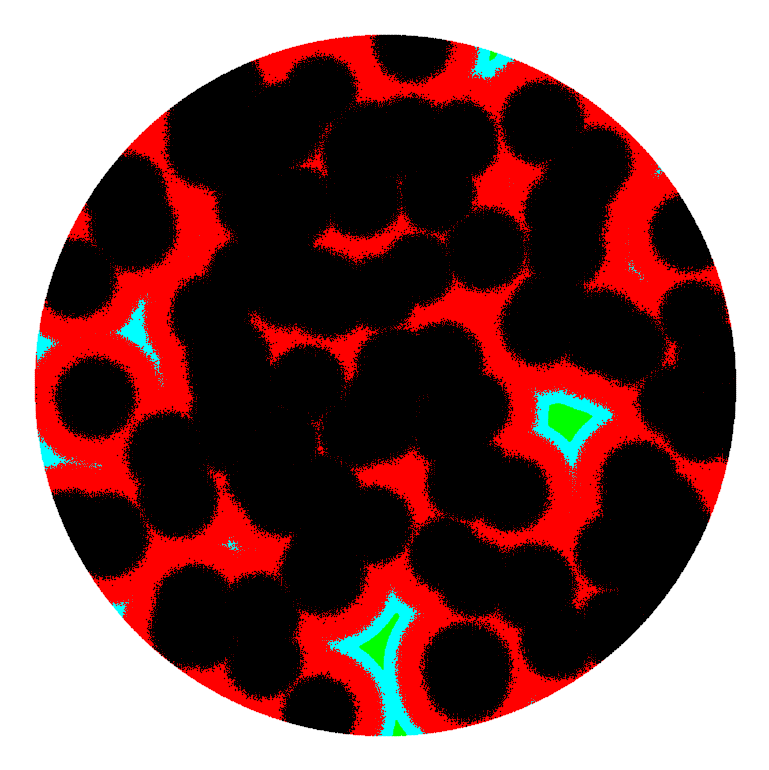
\includegraphics[width=0.48\textwidth]{Figures/Full-Dish-CellPhotos/cell79.png}
        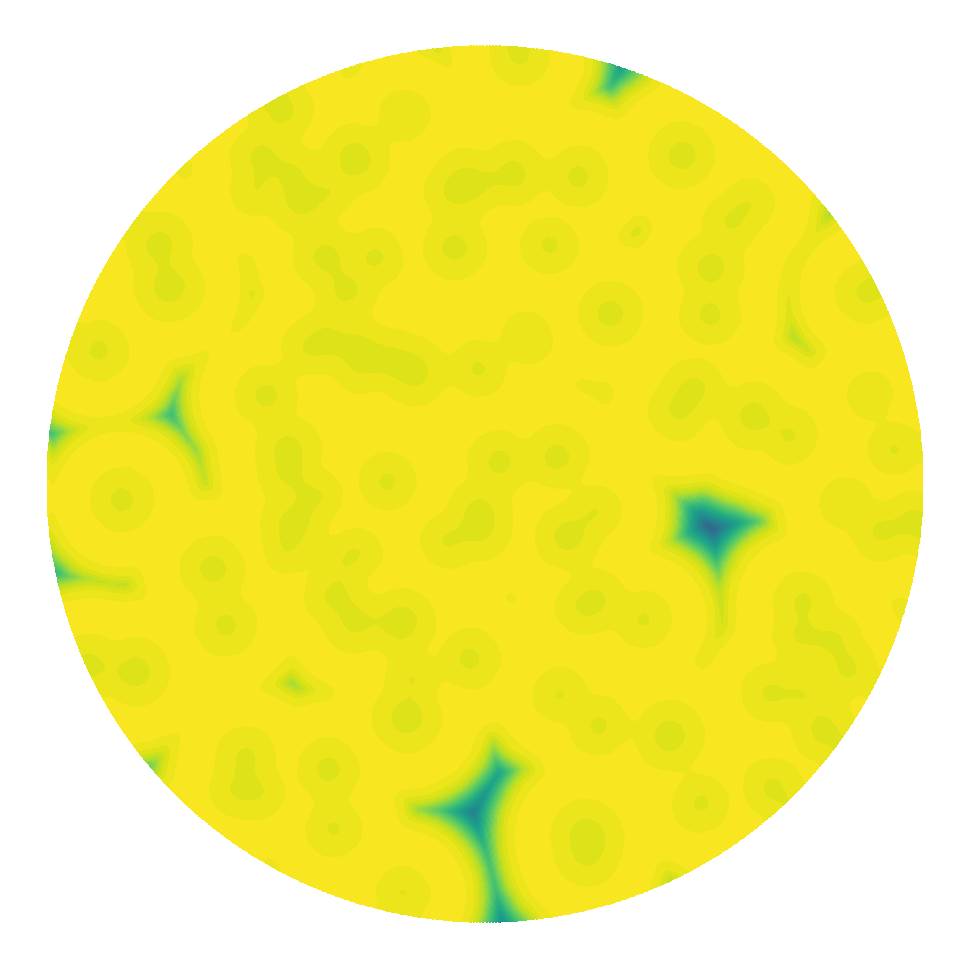
\includegraphics[width=0.48\textwidth]{Figures/Full-Dish-VirusPhotos/virus79.png}}

    \resizebox{0.48\textwidth}{!}{% 
        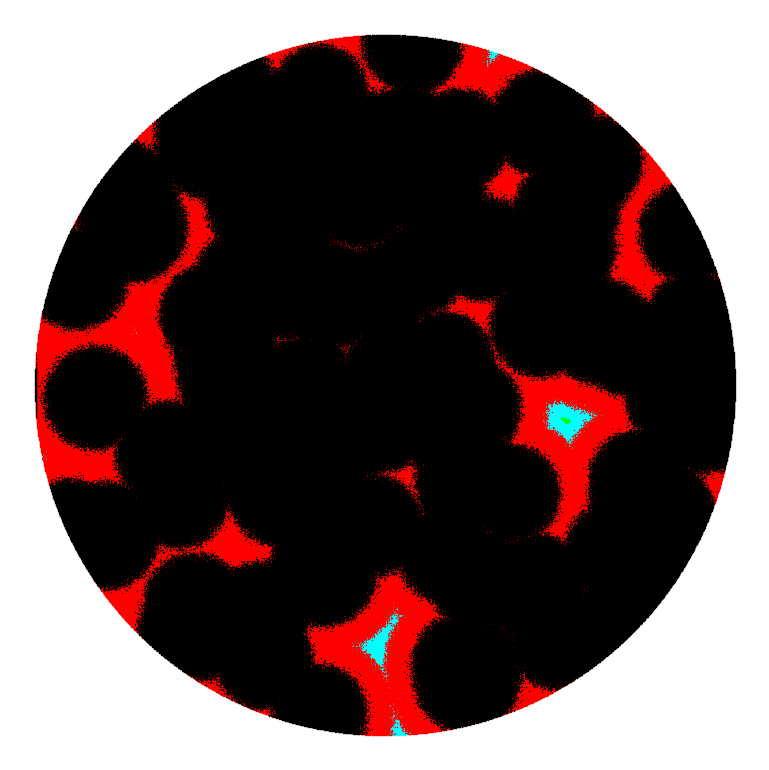
\includegraphics[width=0.48\textwidth]{Figures/Full-Dish-CellPhotos/cell89.png}
        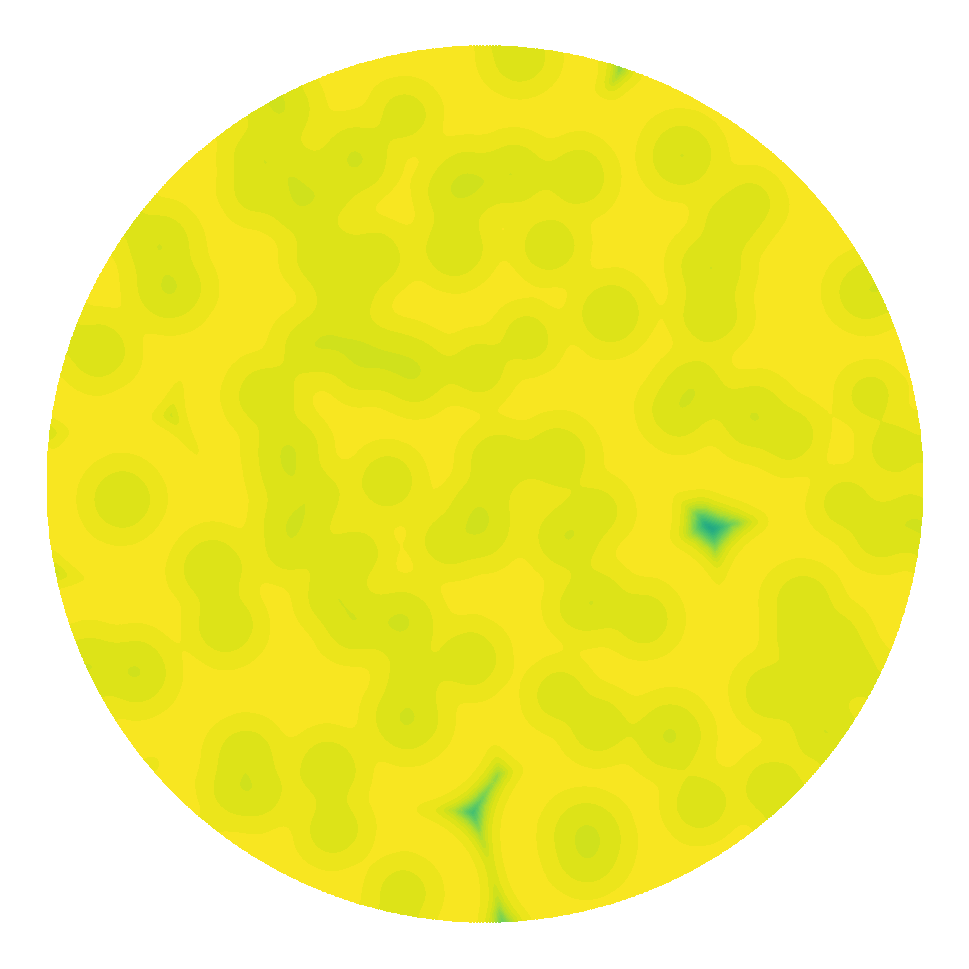
\includegraphics[width=0.48\textwidth]{Figures/Full-Dish-VirusPhotos/virus89.png}}

    \resizebox{0.48\textwidth}{!}{%
        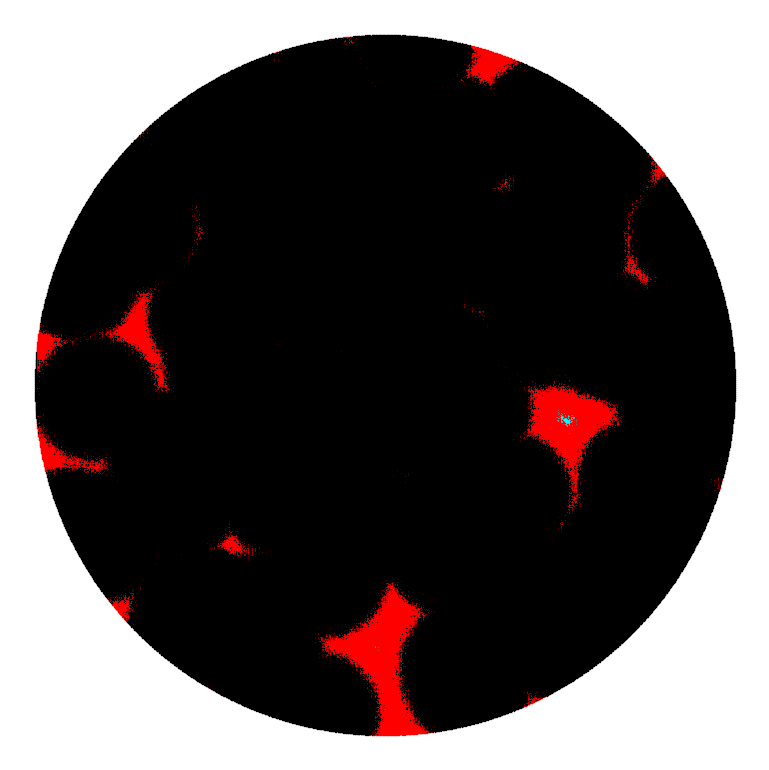
\includegraphics[width=0.48\textwidth]{Figures/Full-Dish-CellPhotos/cell99.png}
        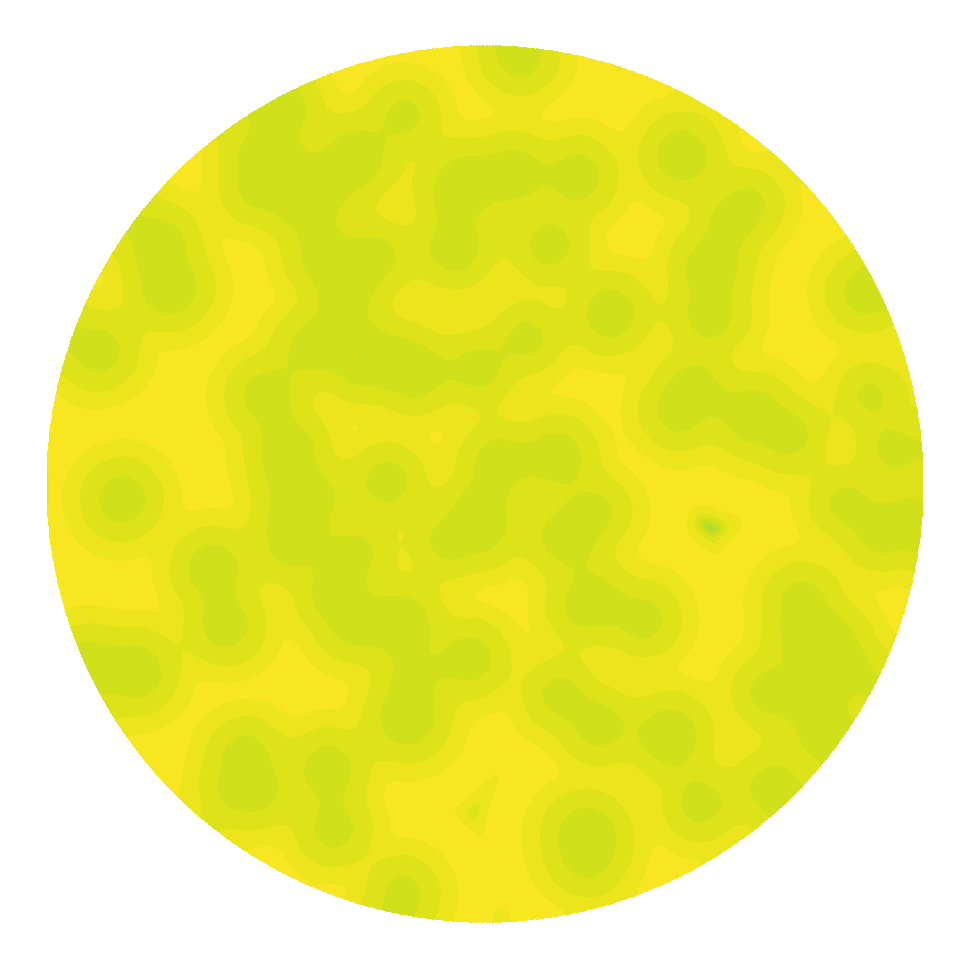
\includegraphics[width=0.48\textwidth]{Figures/Full-Dish-VirusPhotos/virus99.png}}

    \resizebox{0.48\textwidth}{!}{%
        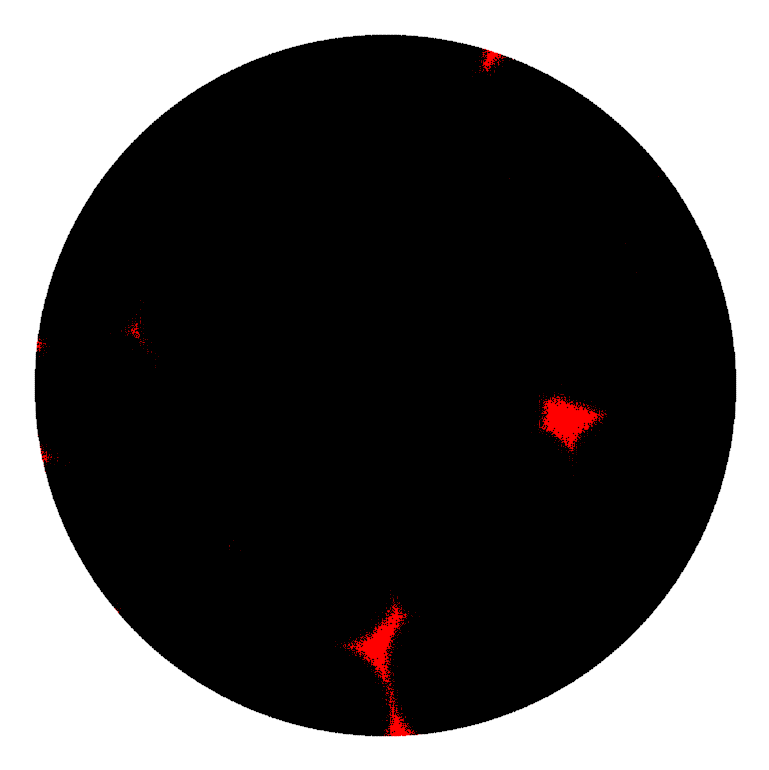
\includegraphics[width=0.48\textwidth]{Figures/Full-Dish-CellPhotos/cell109.png}
        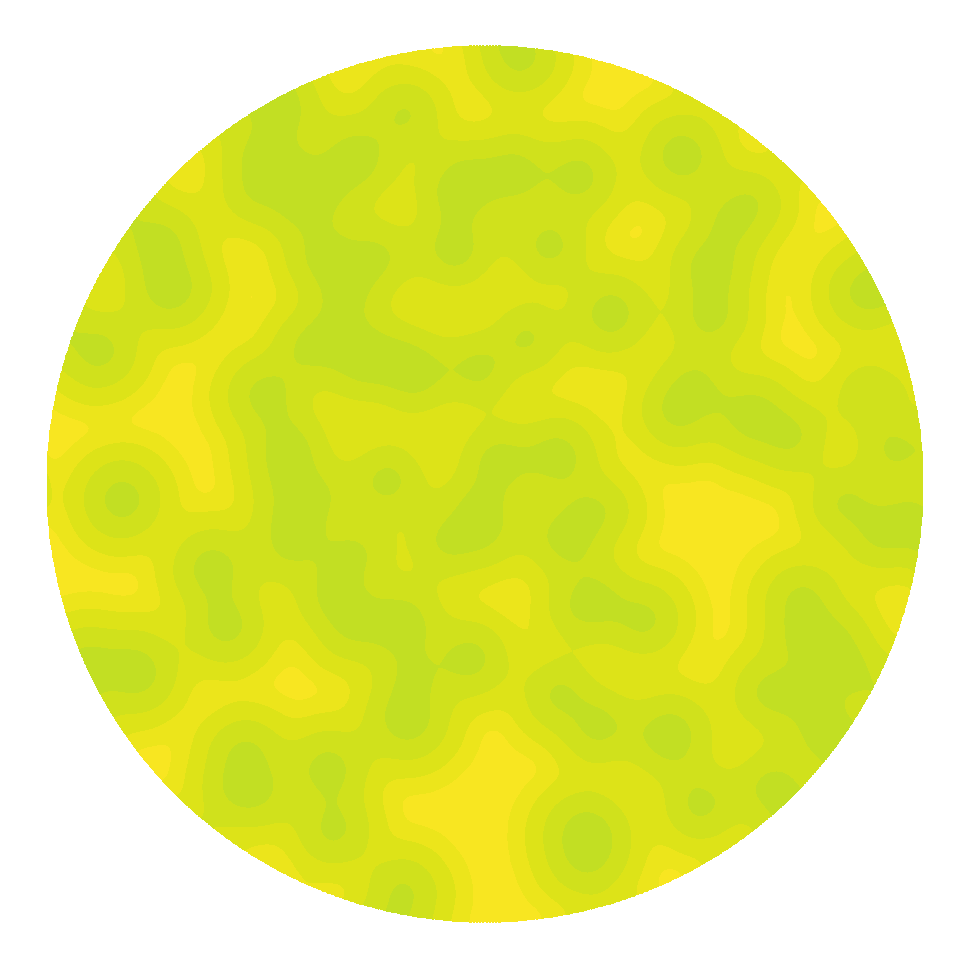
\includegraphics[width=0.48\textwidth]{Figures/Full-Dish-VirusPhotos/virus109.png}}

    \resizebox{0.48\textwidth}{!}{%
        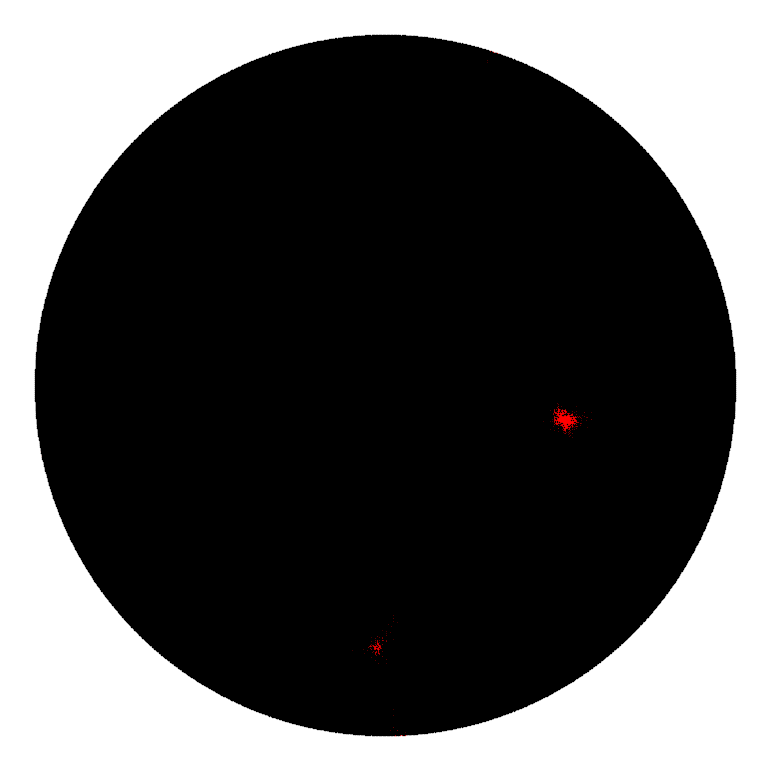
\includegraphics[width=0.48\textwidth]{Figures/Full-Dish-CellPhotos/cell119.png}
        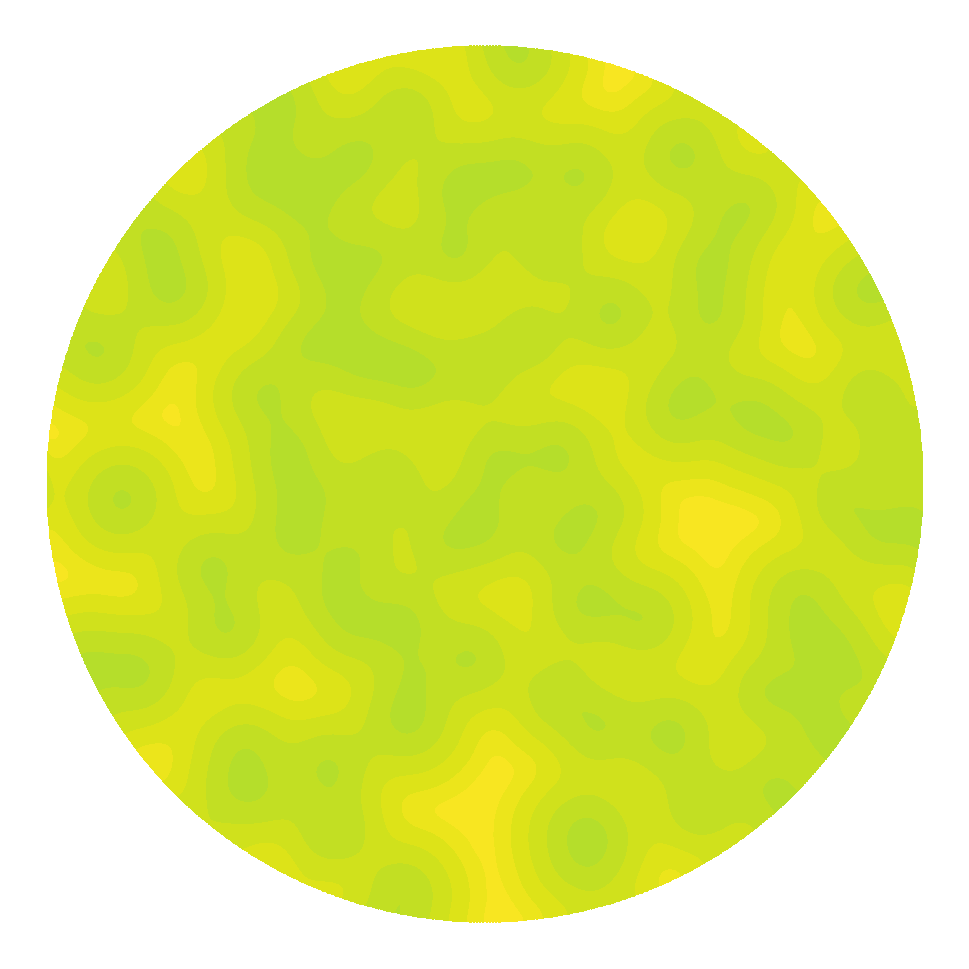
\includegraphics[width=0.48\textwidth]{Figures/Full-Dish-VirusPhotos/virus119.png}}

\end{multicols}
\end{minipage}
\caption{The dish at hours 5 through 60 in 5 hour increments. On the left are cells in the different stages of infection; the stages are represented by healthy cells colored green, eclipse cells colored cyan, infected cells colored red, and dead cells colored black. On the right are images of the virions that are diffusing over the cells; areas of higher concentration are represented by yellow and areas of lower concentration are represented by purple. \label{fig_FullDish_cellandvirus}}
\end{figure}

\begin{figure}
\centering
\begin{minipage}{0.66\linewidth}
\centering
    \resizebox{\textwidth}{!}{%
        
\includegraphics[width=0.48\textwidth]{Figures/Zoomed-In-CellPhotos/cell12.png}
        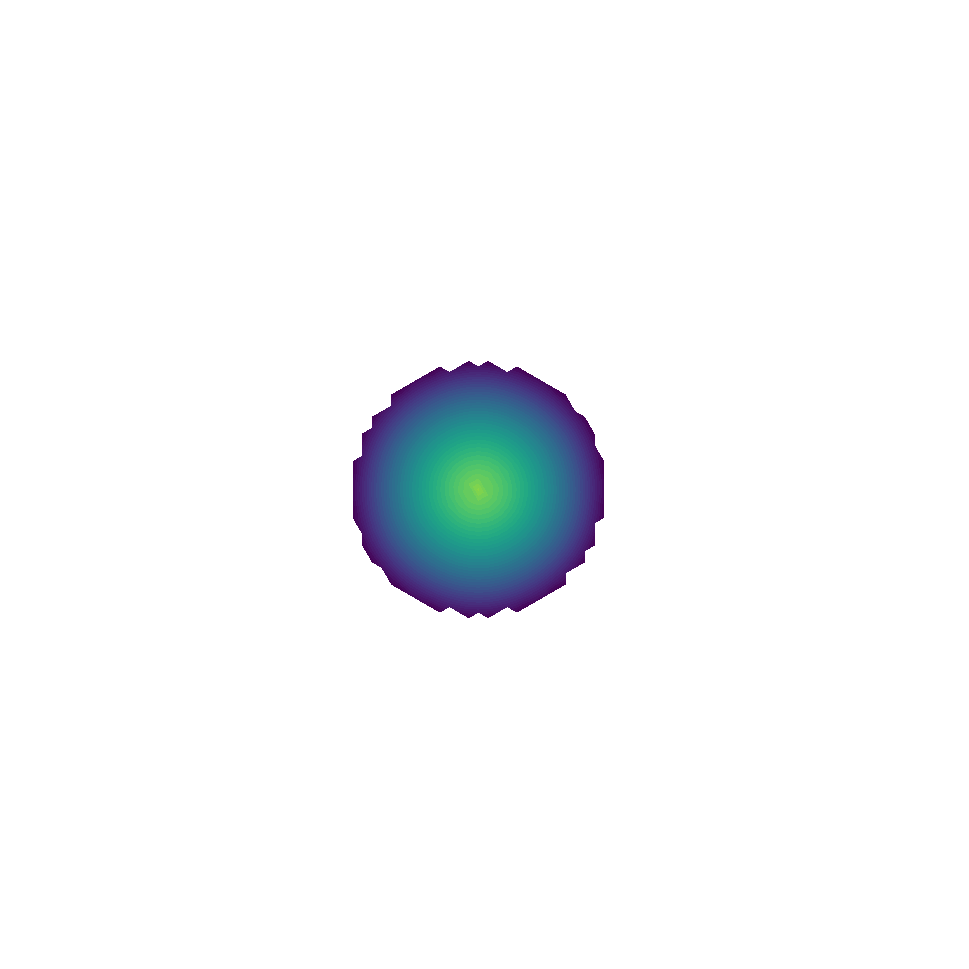
\includegraphics[width=0.48\textwidth]{Figures/Zoomed-In-VirusPhotos/virus12.png}}

    \vspace{0.25em}
    \resizebox{\textwidth}{!}{%
        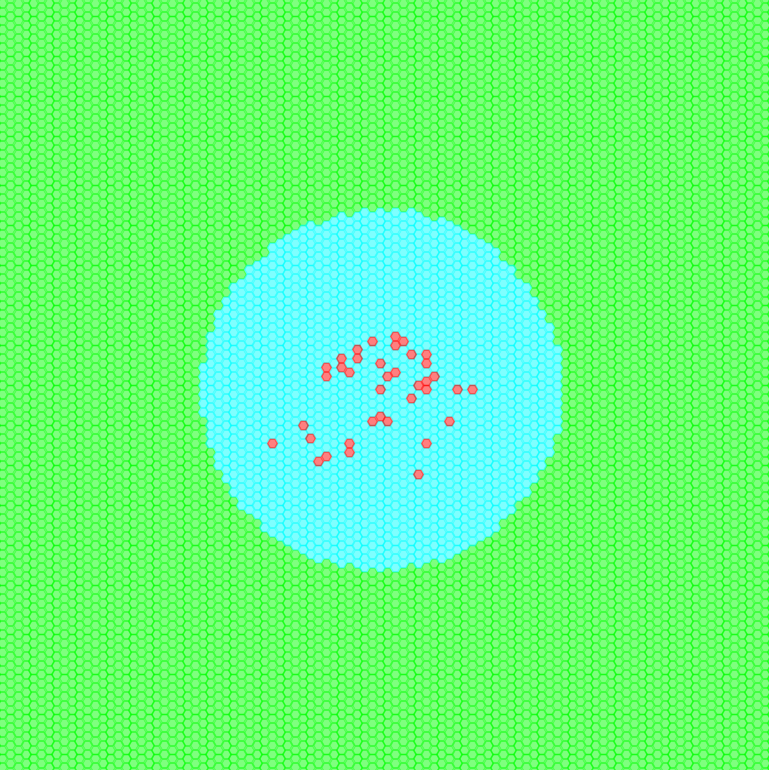
\includegraphics[width=0.48\textwidth]{Figures/Zoomed-In-CellPhotos/cell22.png}
        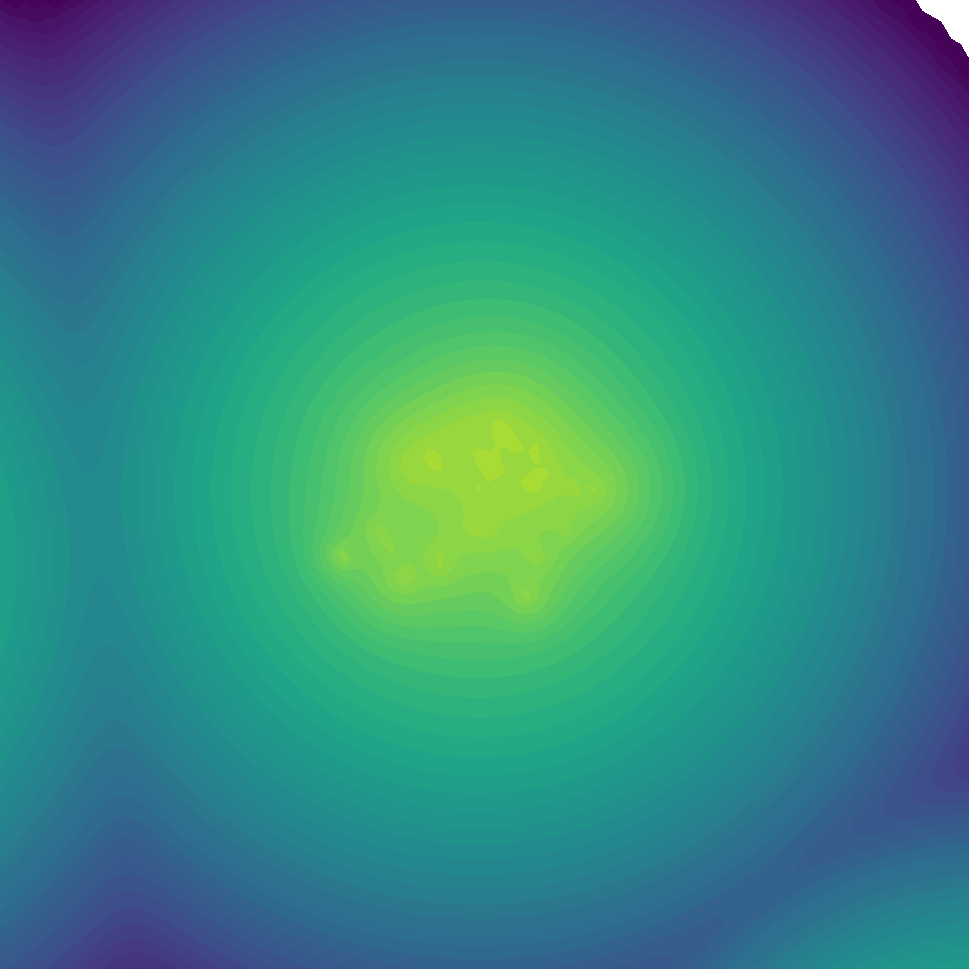
\includegraphics[width=0.48\textwidth]{Figures/Zoomed-In-VirusPhotos/virus22.png}}

    \vspace{0.25em}
    \resizebox{\textwidth}{!}{%
        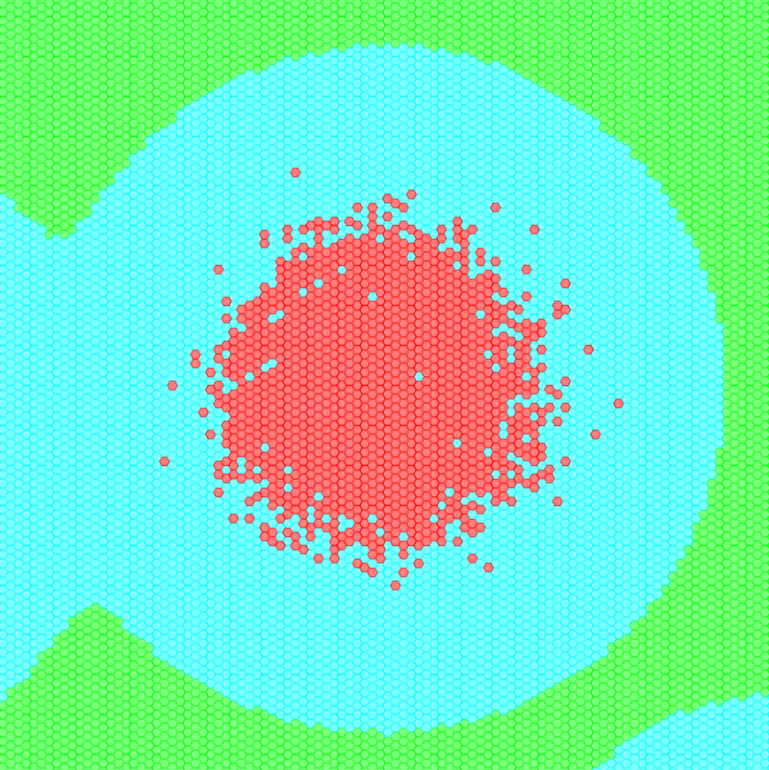
\includegraphics[width=0.48\textwidth]{Figures/Zoomed-In-CellPhotos/cell32.png}
        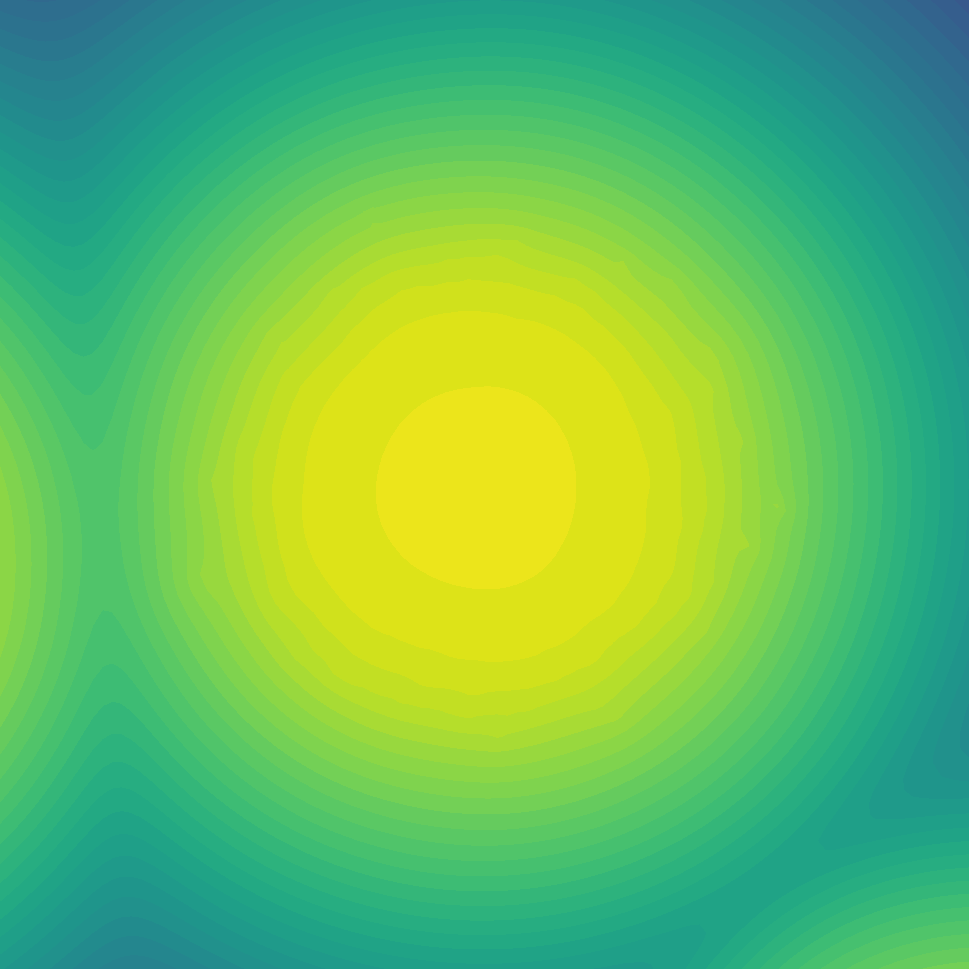
\includegraphics[width=0.48\textwidth]{Figures/Zoomed-In-VirusPhotos/virus32.png}}
\end{minipage}
\caption{A zoomed in section of the dish looking at the plaque formed by a single infected cell during a viral infection at hours 6.5, 11.5, and 16.5. On the left are cells in the different stages of infection; the stages are represented by healthy cells colored green, eclipse cells colored cyan, infected cells colored red, and dead cells colored black. On the right are the many virus that are diffusing over the cells; areas of higher concentration are represented by yellow and areas of lower concentration are represented by purple. \label{fig_ZoominDish}}
\end{figure}


%\begin{figure}
%\captionsetup[subfigure]{aboveskip=-1pt,belowskip=1pt}
%\centering
%\parbox{0.66\textwidth}{%
%    \hspace{-0.6875em}
%    \resizebox{0.33\textwidth}{!}{
\includegraphics{Figures/Zoomed-In-CellPhotos/cell12.png}}
%    \resizebox{0.33\textwidth}{!}{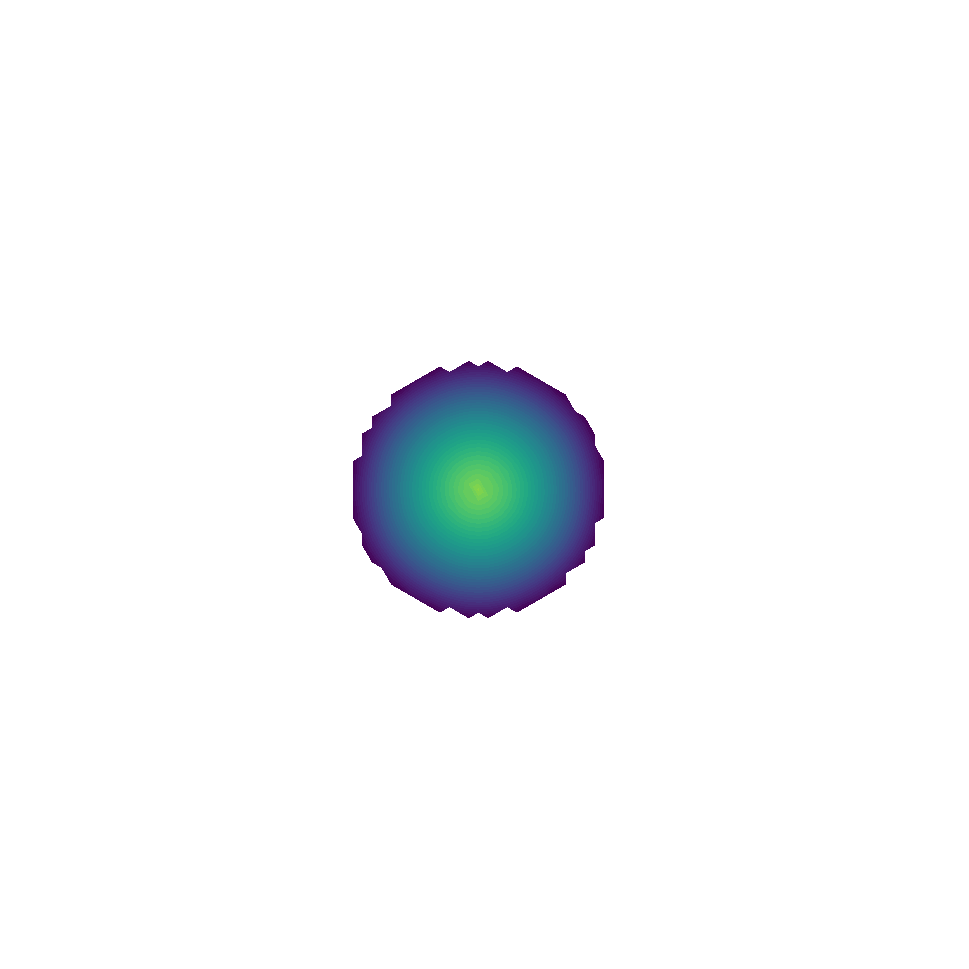
\includegraphics{Figures/Zoomed-In-VirusPhotos/virus12.png}}

%    \vspace{0.25em}
%    \hspace{-0.6875em}
%    \resizebox{0.33\textwidth}{!}{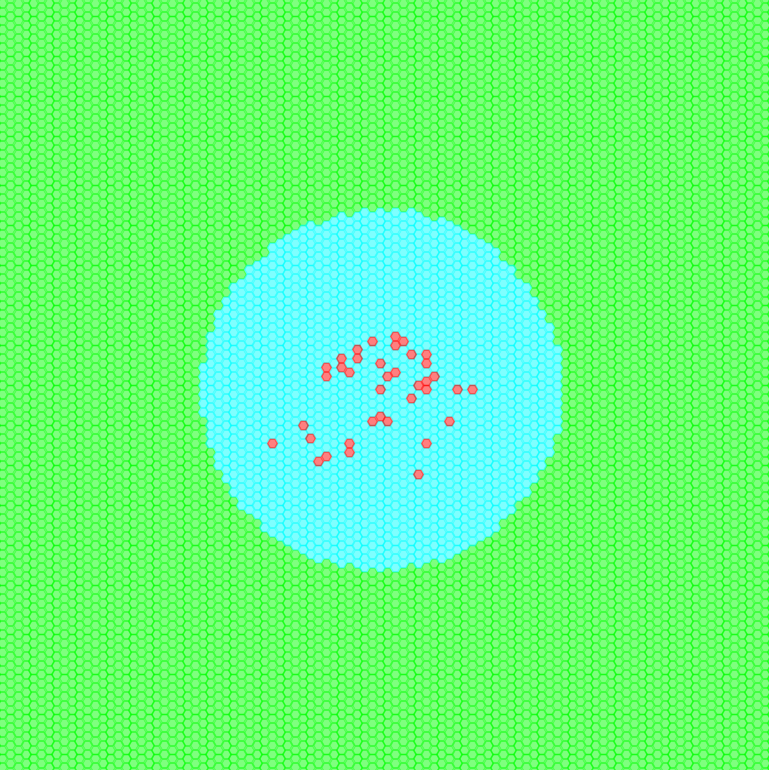
\includegraphics{Figures/Zoomed-In-CellPhotos/cell22.png}}
%    \resizebox{0.33\textwidth}{!}{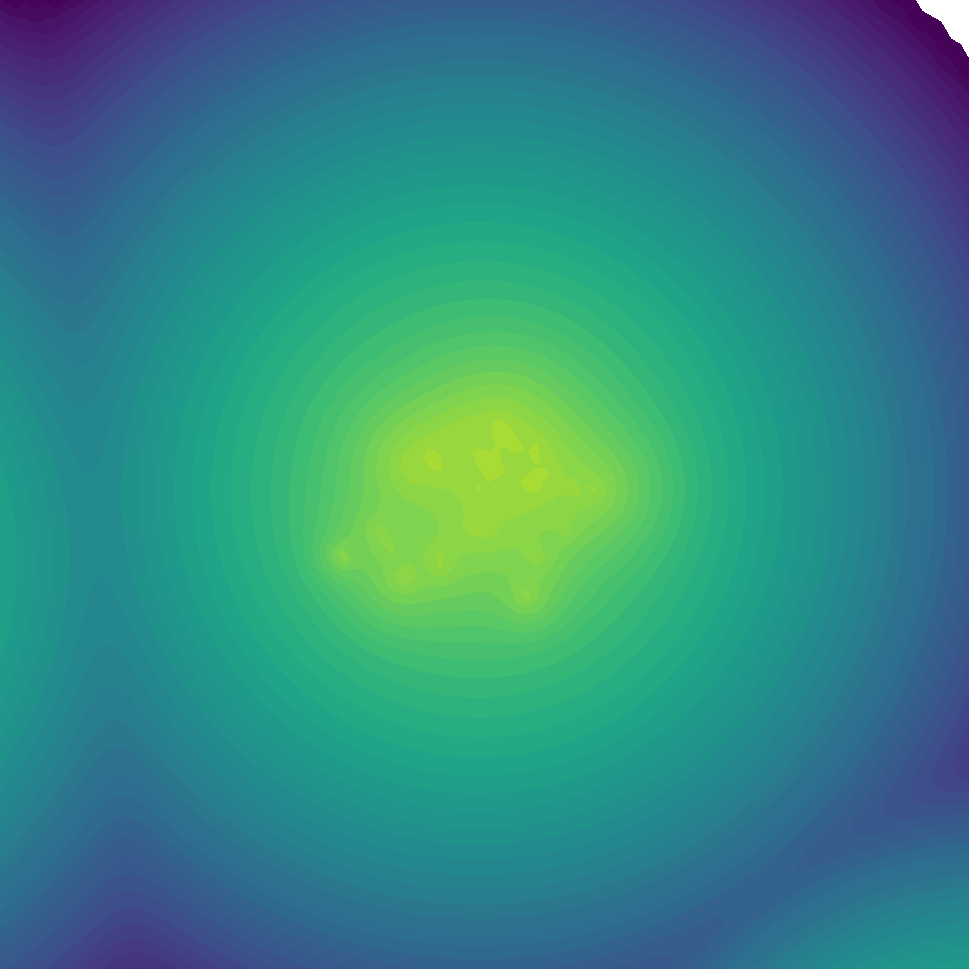
\includegraphics{Figures/Zoomed-In-VirusPhotos/virus22.png}}

%    \vspace{0.25em}
%    \hspace{-0.6875em}
%    \resizebox{0.33\textwidth}{!}{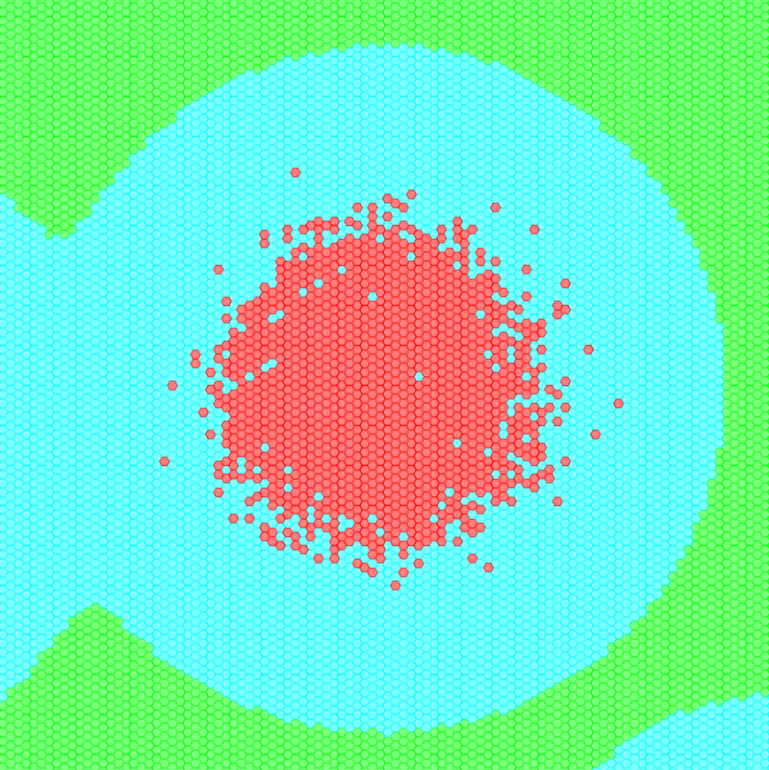
\includegraphics{Figures/Zoomed-In-CellPhotos/cell32.png}}
%    \resizebox{0.33\textwidth}{!}{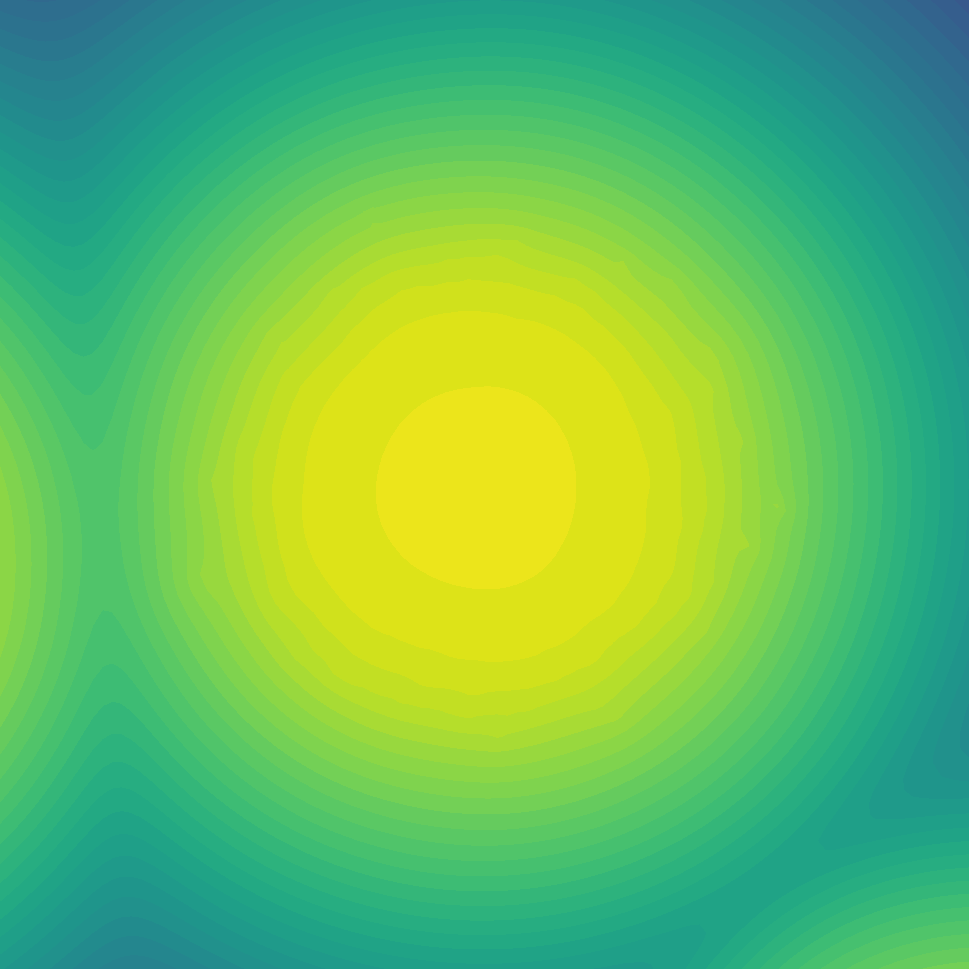
\includegraphics{Figures/Zoomed-In-VirusPhotos/virus32.png}}}

%    \caption{A zoomed in section of the dish looking at the plaque formed by a single infected cell during a viral infection at hours 6.5, 11.5, and 16.5. On the left are cells in the different stages of infection; the stages are represented by healthy cells colored green, eclipse cells colored cyan, infected cells colored red, and dead cells colored black. On the right are the many virus that are diffusing over the cells; areas of higher concentration are represented by yellow and areas of lower concentration are represented by purple. \label{fig_ZoominDish}}
%\end{figure}

%\clearpage
\subsection{Implementation on GPUs}

We simulated ten viral infections for five different numbers of cells, with codes that utilize three different programming languages: Python, C, and CUDA. The amount of computation time needed to simulate one hour of the infection, on a desktop computer, is shown in figure \ref{fig:SpeedComparison}. The computer was built with an Intel Xeon E-2144G CPU, 16 gigabytes of RAM, and P4000 Nvidia Graphics card. The compute times for the three codes increase as the number of cells in the simulations increases, but the speed increase of switching from Python, the programming language commonly used in physics, to code using CUDA for implementation on GPUs is 6954 times faster.
\begin{figure}
    \centering
    \resizebox{0.6\textwidth}{!}{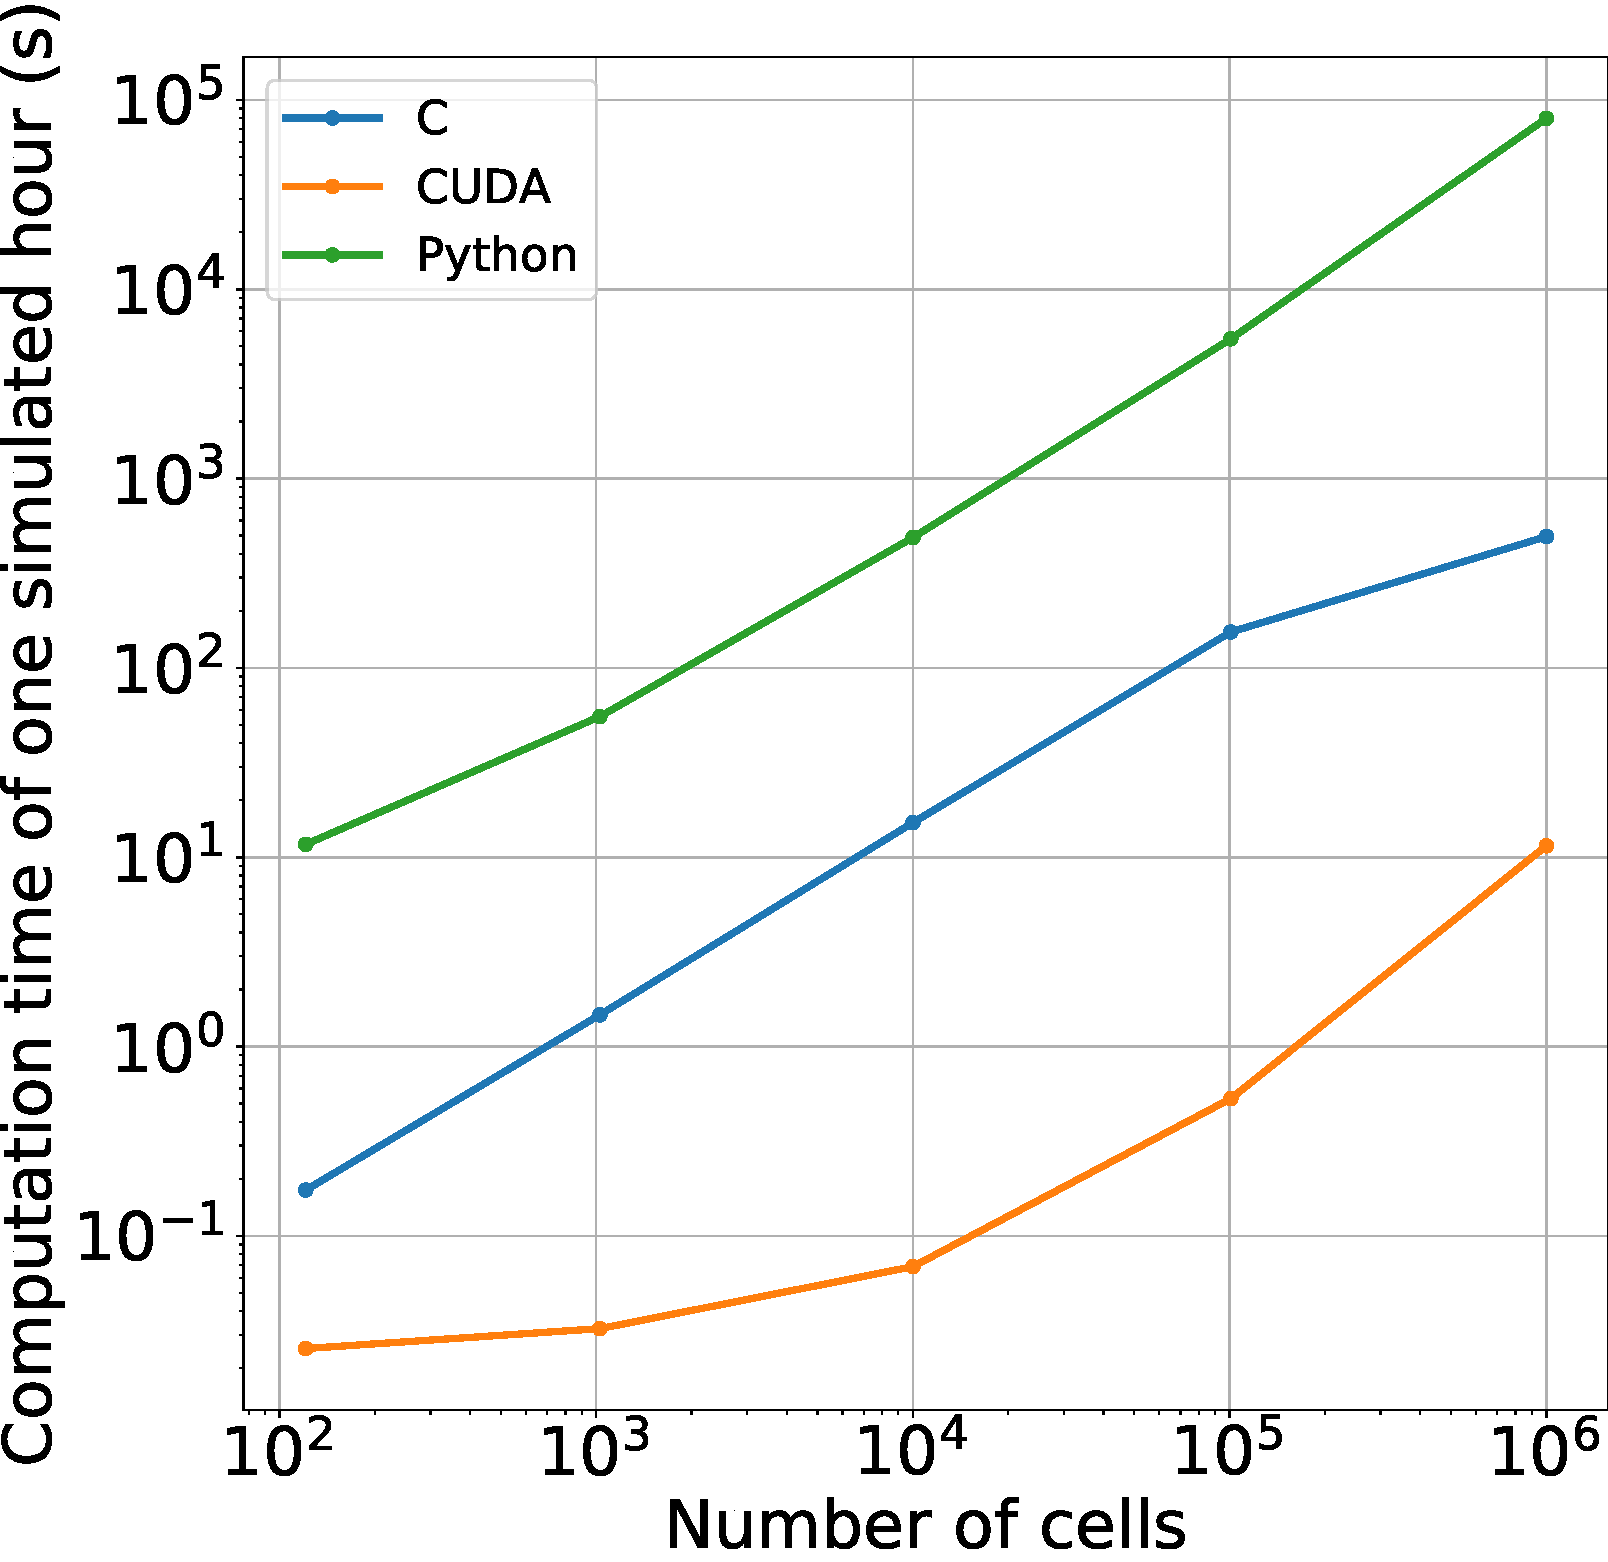
\includegraphics{Figures/loglogspeed.pdf}}
\caption{With more than a million cells, CUDA is 6954 times faster then the Python code and 43 time faster than the C code. \label{fig:SpeedComparison}}
\end{figure}

%\clearpage
\subsection{Convergence Testing}

We examine three scenarios when testing the convergence of the model: an infection initiated with $10013$ cells in the eclipse phase (Initial Cell); an infection initiated with $10^{12}$ virions (Initial Virus); and a scenario with no infection, but $10^{12}$ virions (Only Virus), examining viral spread and decay only. Simulations in each of the scenarios used the influenza parameters from Table \ref{tab_params}. Figure \ref{fig:ViralTiterCurves} shows the simulations of the three scenarios, where the time step was varied to test the convergence of the model in time. A time step of 0.005 hr was chosen and a range around it was made by dividing or multiplying by 2 repeatedly. This formed an array of seven time step values, 0.000625, 0.00128, 0.0025, 0.005, 0.01, 0.02, and 0.04 hr. For each time step, the median curve of ten viral titer curves is shown. In figure \ref{fig:ViralTiterCurves}, from left to right, curves of a viral infection initiated with infected cells; curves of a viral infection initiated with virus; and curves of virus without underlying cell infection. We see that for all the time steps, except $0.04$ hr, the curves are hard to distinguish from one another and follow the same trend for each scenario. 

\begin{figure}
    \centering
    \parbox{\textwidth}{
    \fbox{\parbox{\textwidth}{\vspace{-1em}
    \begin{multicols}{3}
        \centering

        Initial Cell

        Initial Virus

        Only Virus
    \end{multicols}
    \vspace{-1em}}}

    \vspace{0.5em}
    \centering
    \resizebox{0.32\textwidth}{!}{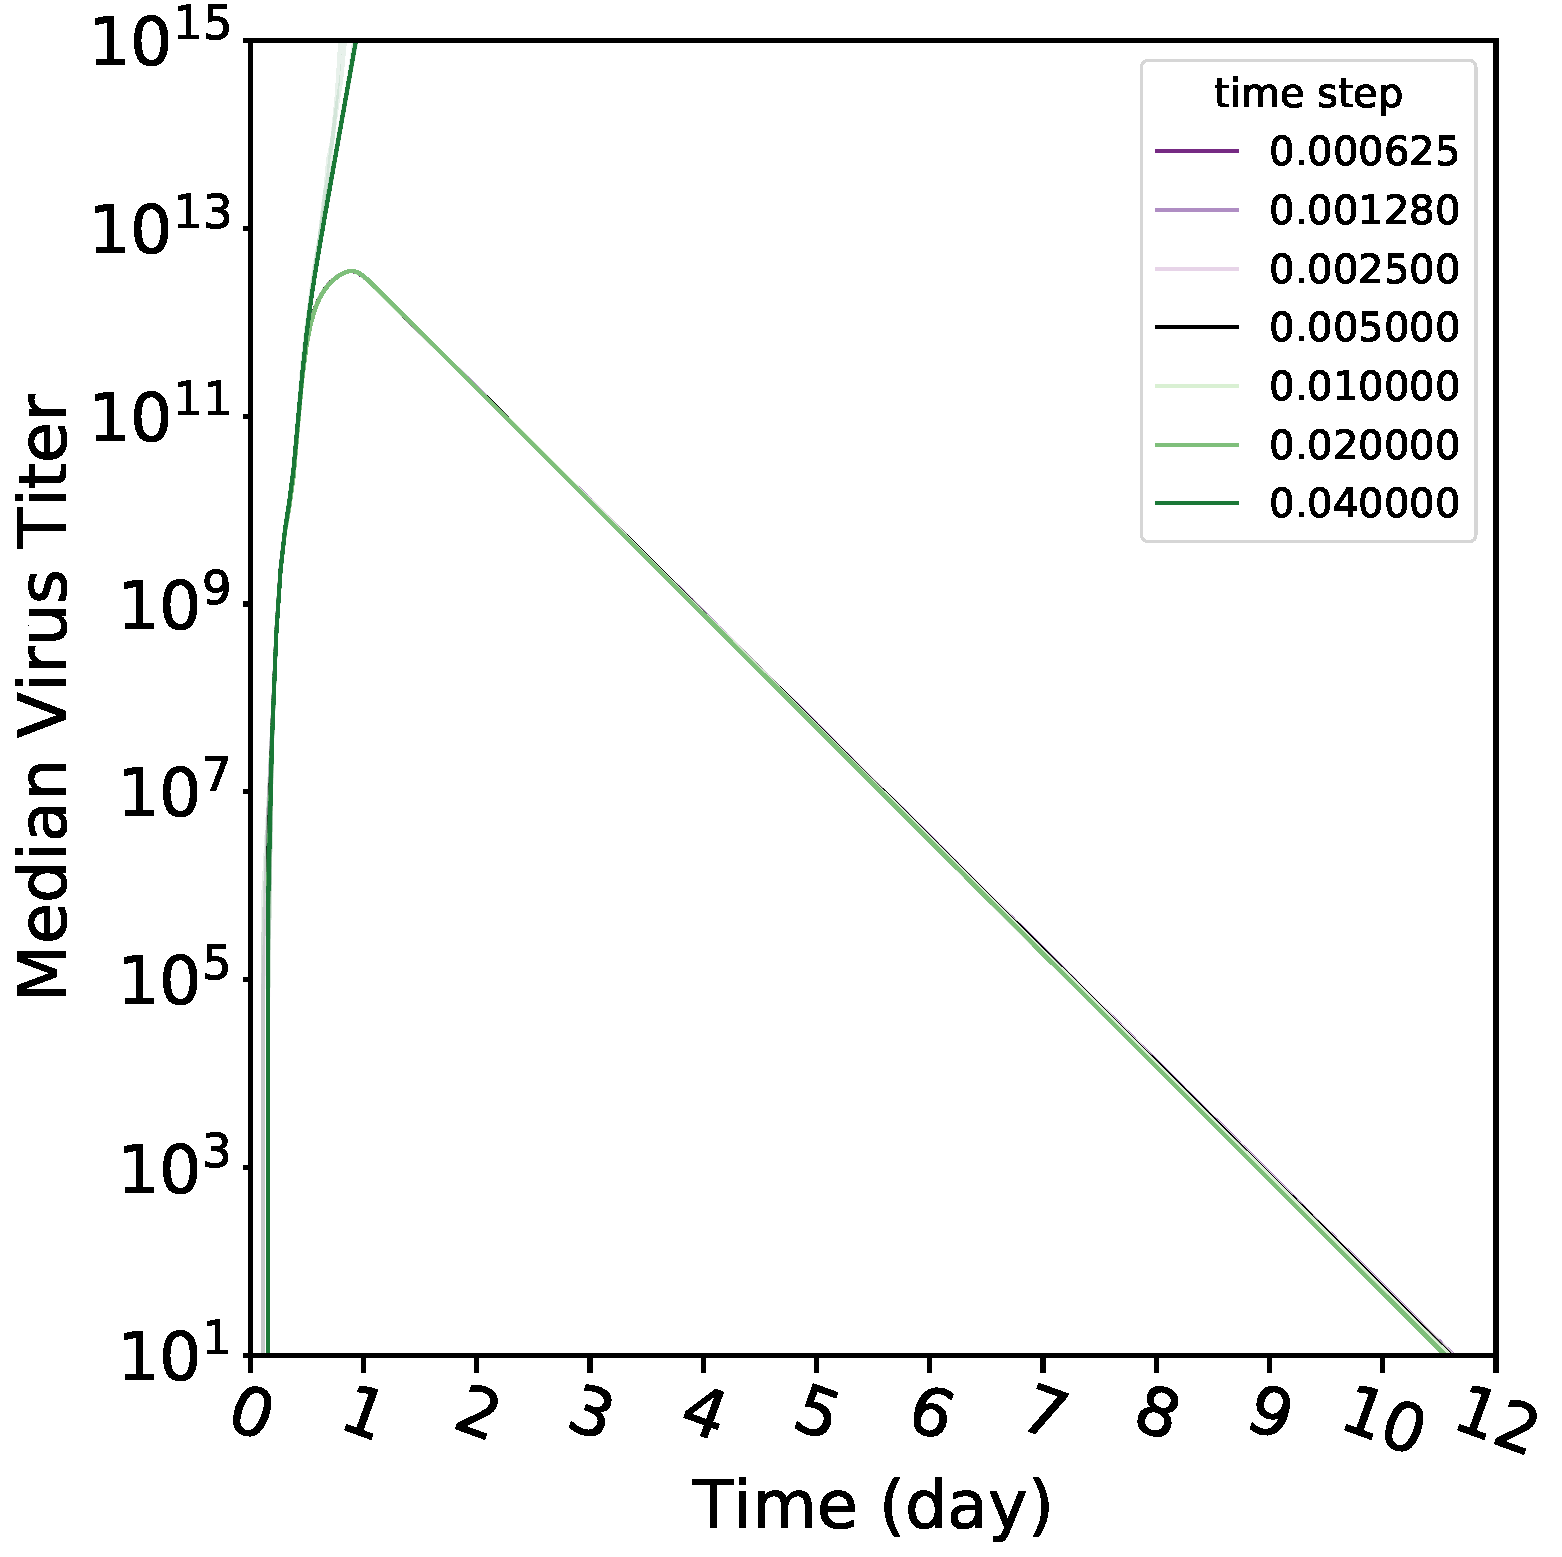
\includegraphics{Figures/Cellfree-InitialCell-AllOnOne_Median_VirusVsTime.pdf}}
    \resizebox{0.32\textwidth}{!}{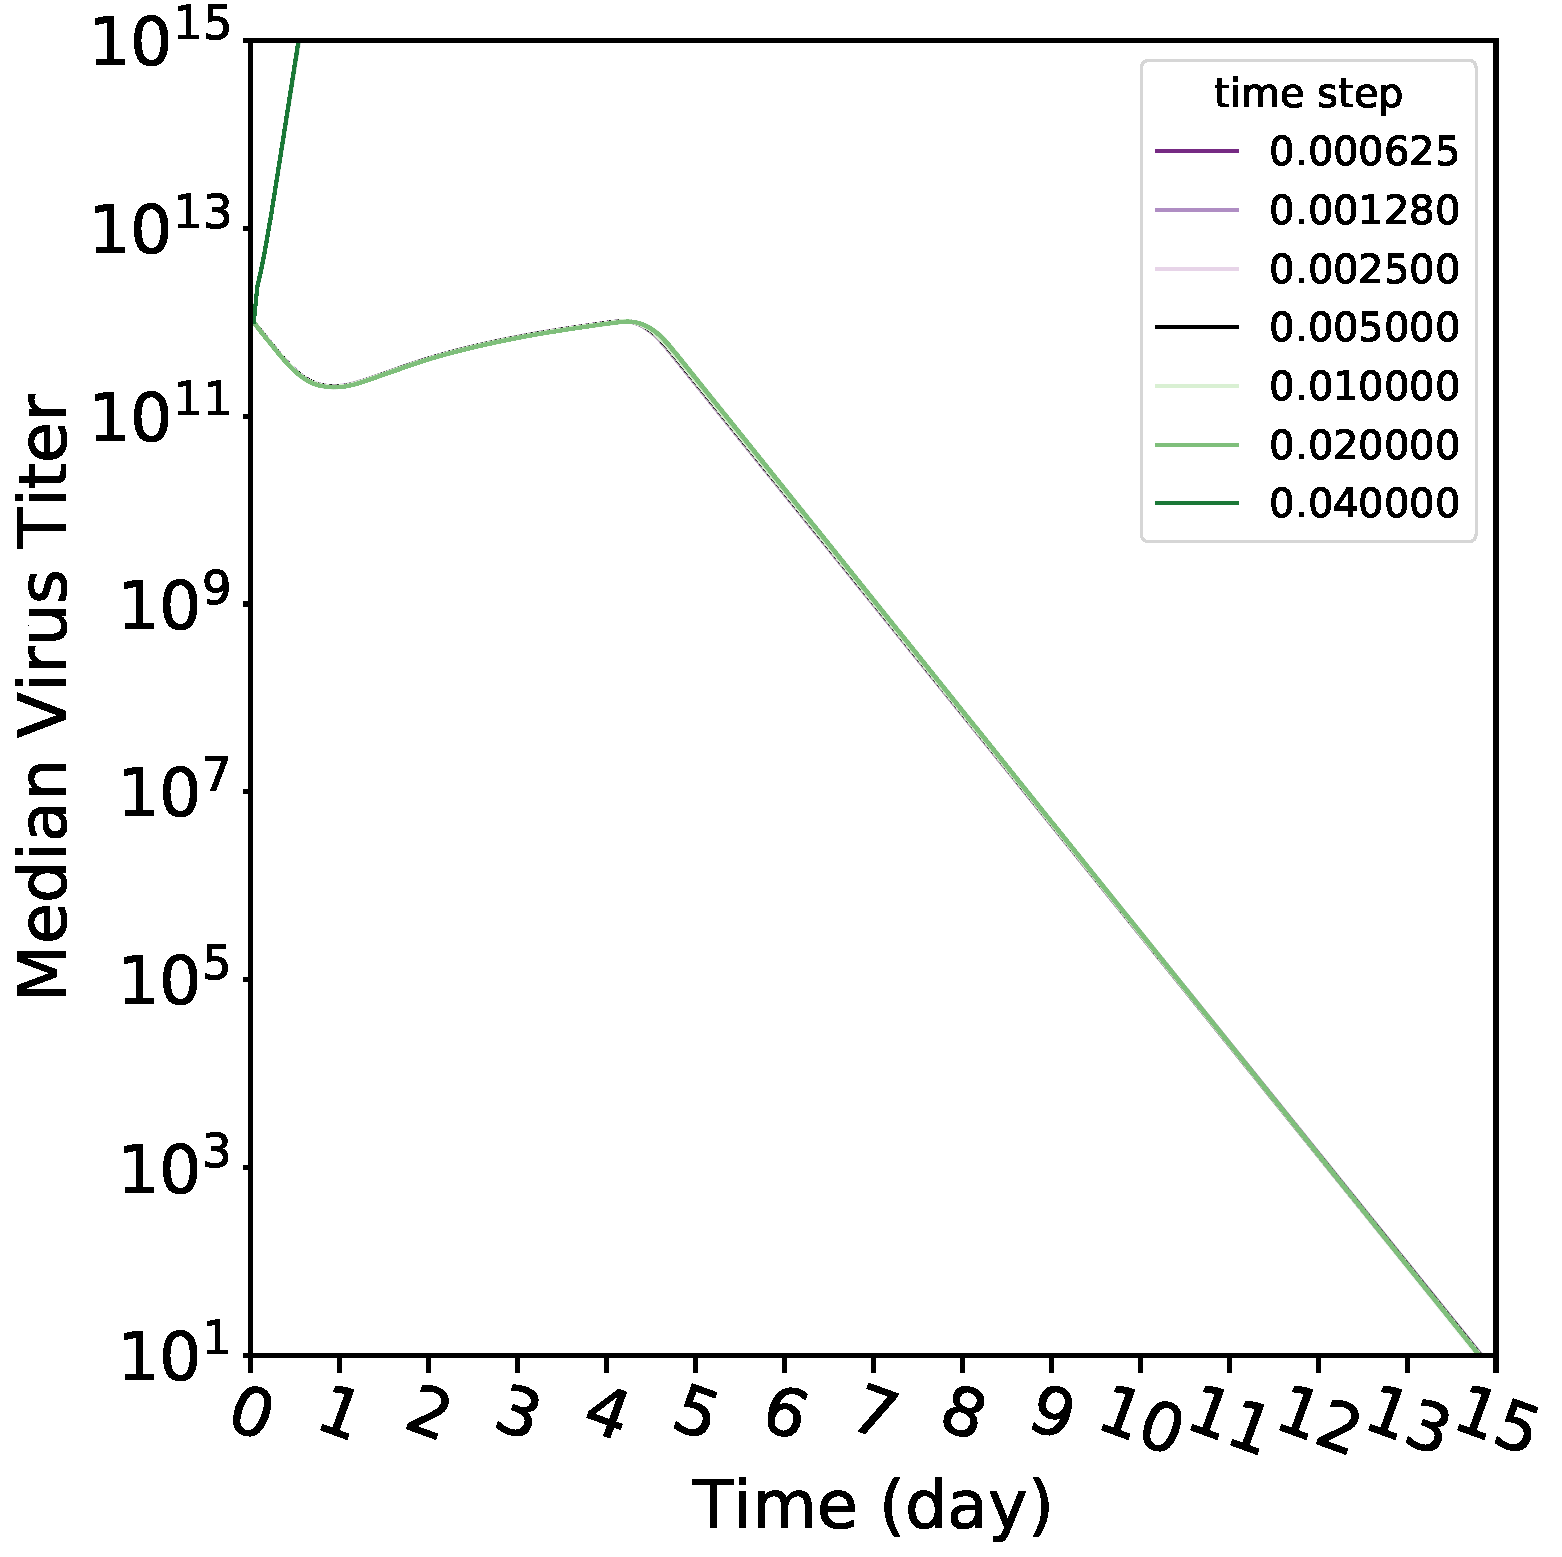
\includegraphics{Figures/Cellfree-InitialVirus-AllOnOne_Median_VirusVsTime.pdf}}
    \resizebox{0.32\textwidth}{!}{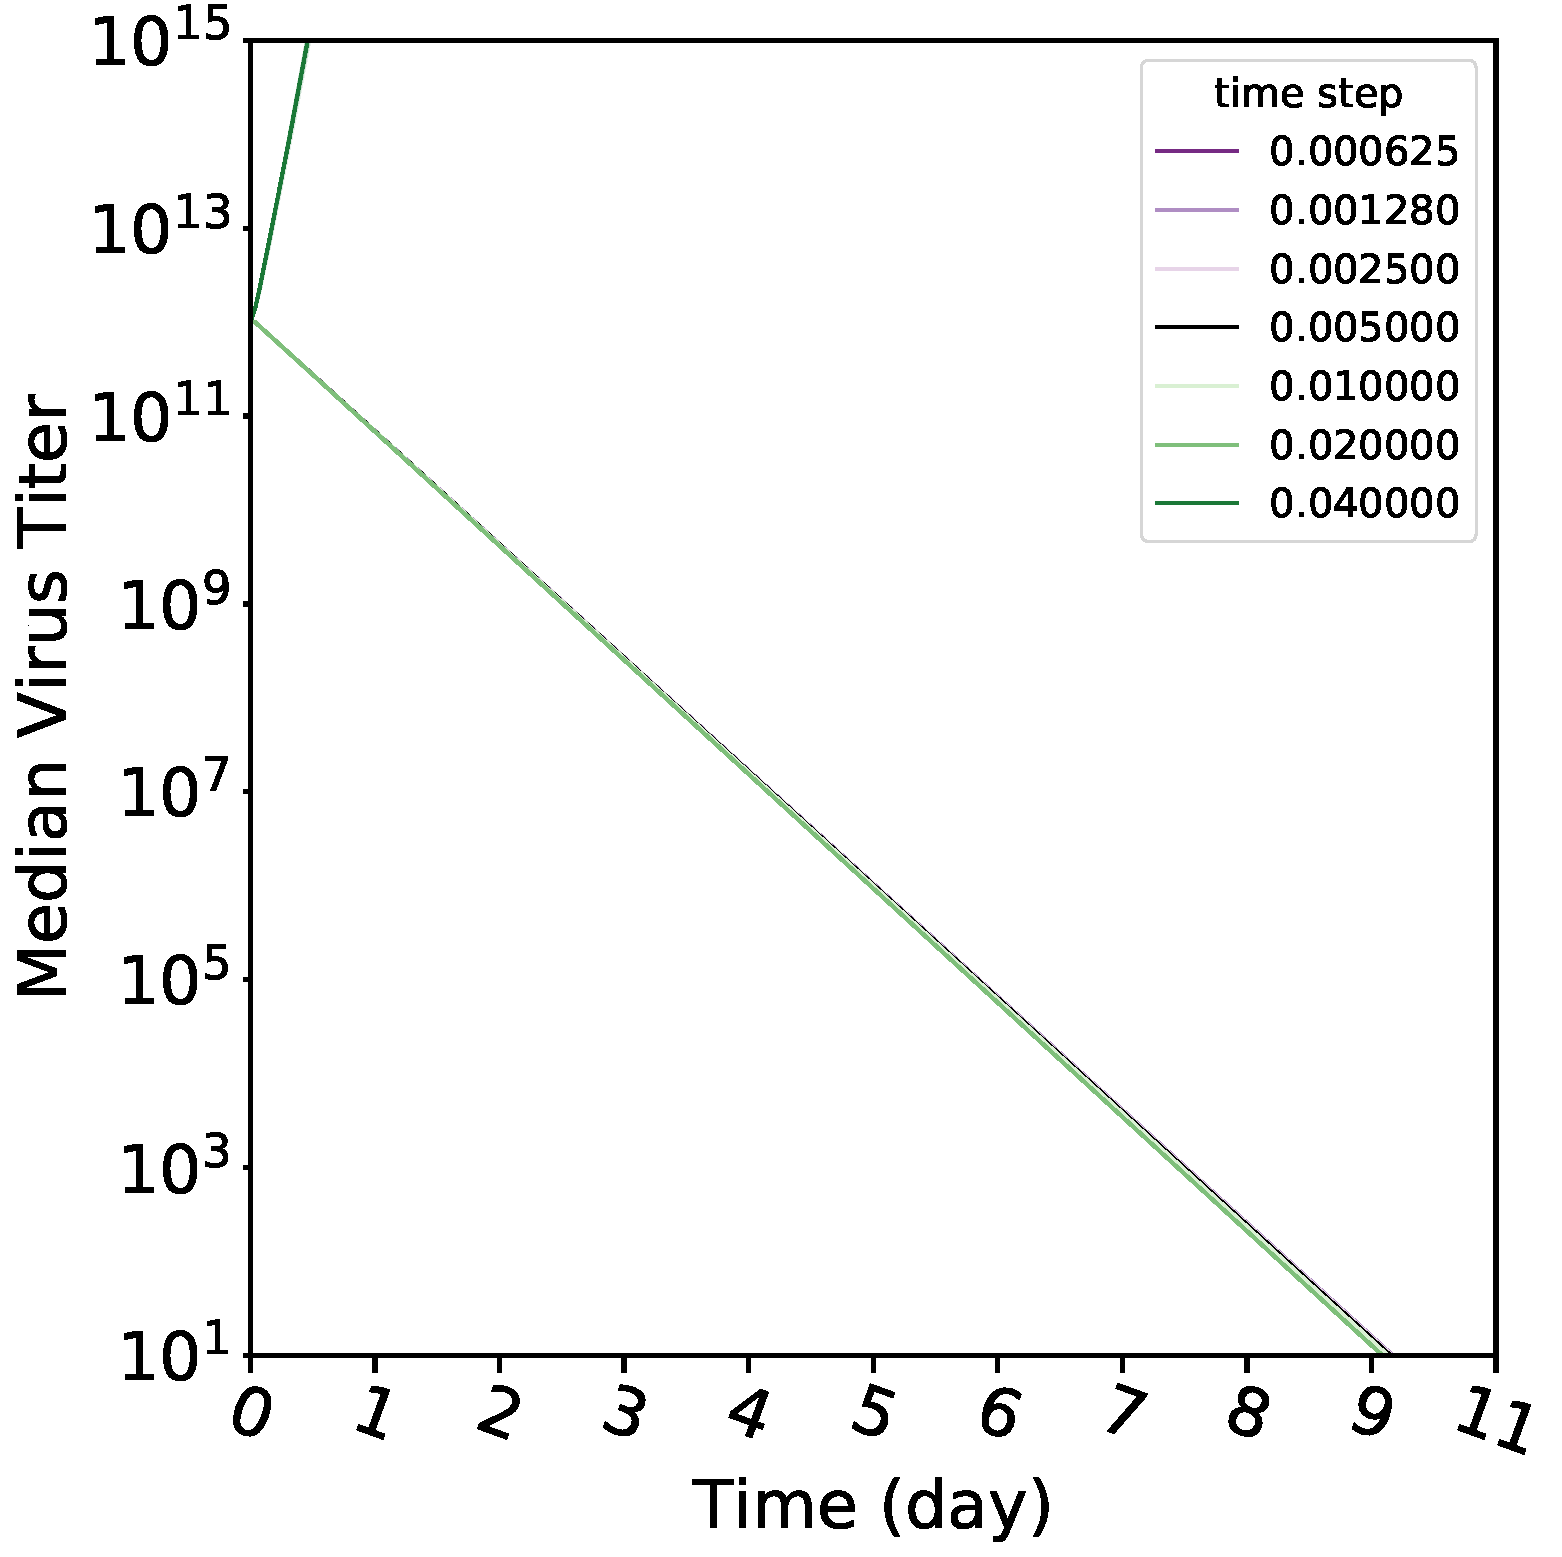
\includegraphics{Figures/Neither-InitialVirus-AllOnOne_Median_VirusVsTime.pdf}}}

\caption{The time step was varied to test the convergence of the model in time. A time step of 0.005 hr was chosen and a range around it was made by dividing or multiplying by 2 repeatedly. Seven values were used [0.000625, 0.00128, 0.0025, 0.005, 0.01, 0.02, 0.04]. The median curve of ten viral titer curves is shown for each time step. From left to right, curves of a viral infection exhibiting cell-free transmission initiated with infected cells; curves of a viral infection exhibiting cell-free transmission initiated with virus; and curves of virus without underlying cell infection. \label{fig:ViralTiterCurves}}
\end{figure}

In figure \ref{fig_AspectGraphs} we explored the different viral titer curves further by plotting the measurable characteristics mentioned in section \ref{Viral_transmission} for each time step. We see very little change in any of the measured quantities until we reach the largest time step. \color{blue} I need to say something about the aspect graphs but I'm not sure what to say. \color{black} \color{red} I think we should take out this figure. It really doesn't add much. Leave it for the thesis.\color{black}

\begin{figure}
%\captionsetup[subfigure]{aboveskip=-1pt,belowskip=1pt}
\centering
\begin{minipage}{\linewidth}
    \centering

    \fbox{\parbox{\textwidth}{\vspace{-1em}
    \begin{multicols}{3}
        \centering

        Initial Cell

        Initial Virus

        Only Virus
    \end{multicols}
    \vspace{-1em}}}

    \vspace{0.5em}

%    \begin{subfigure}[b]{0.3\linewidth}
%        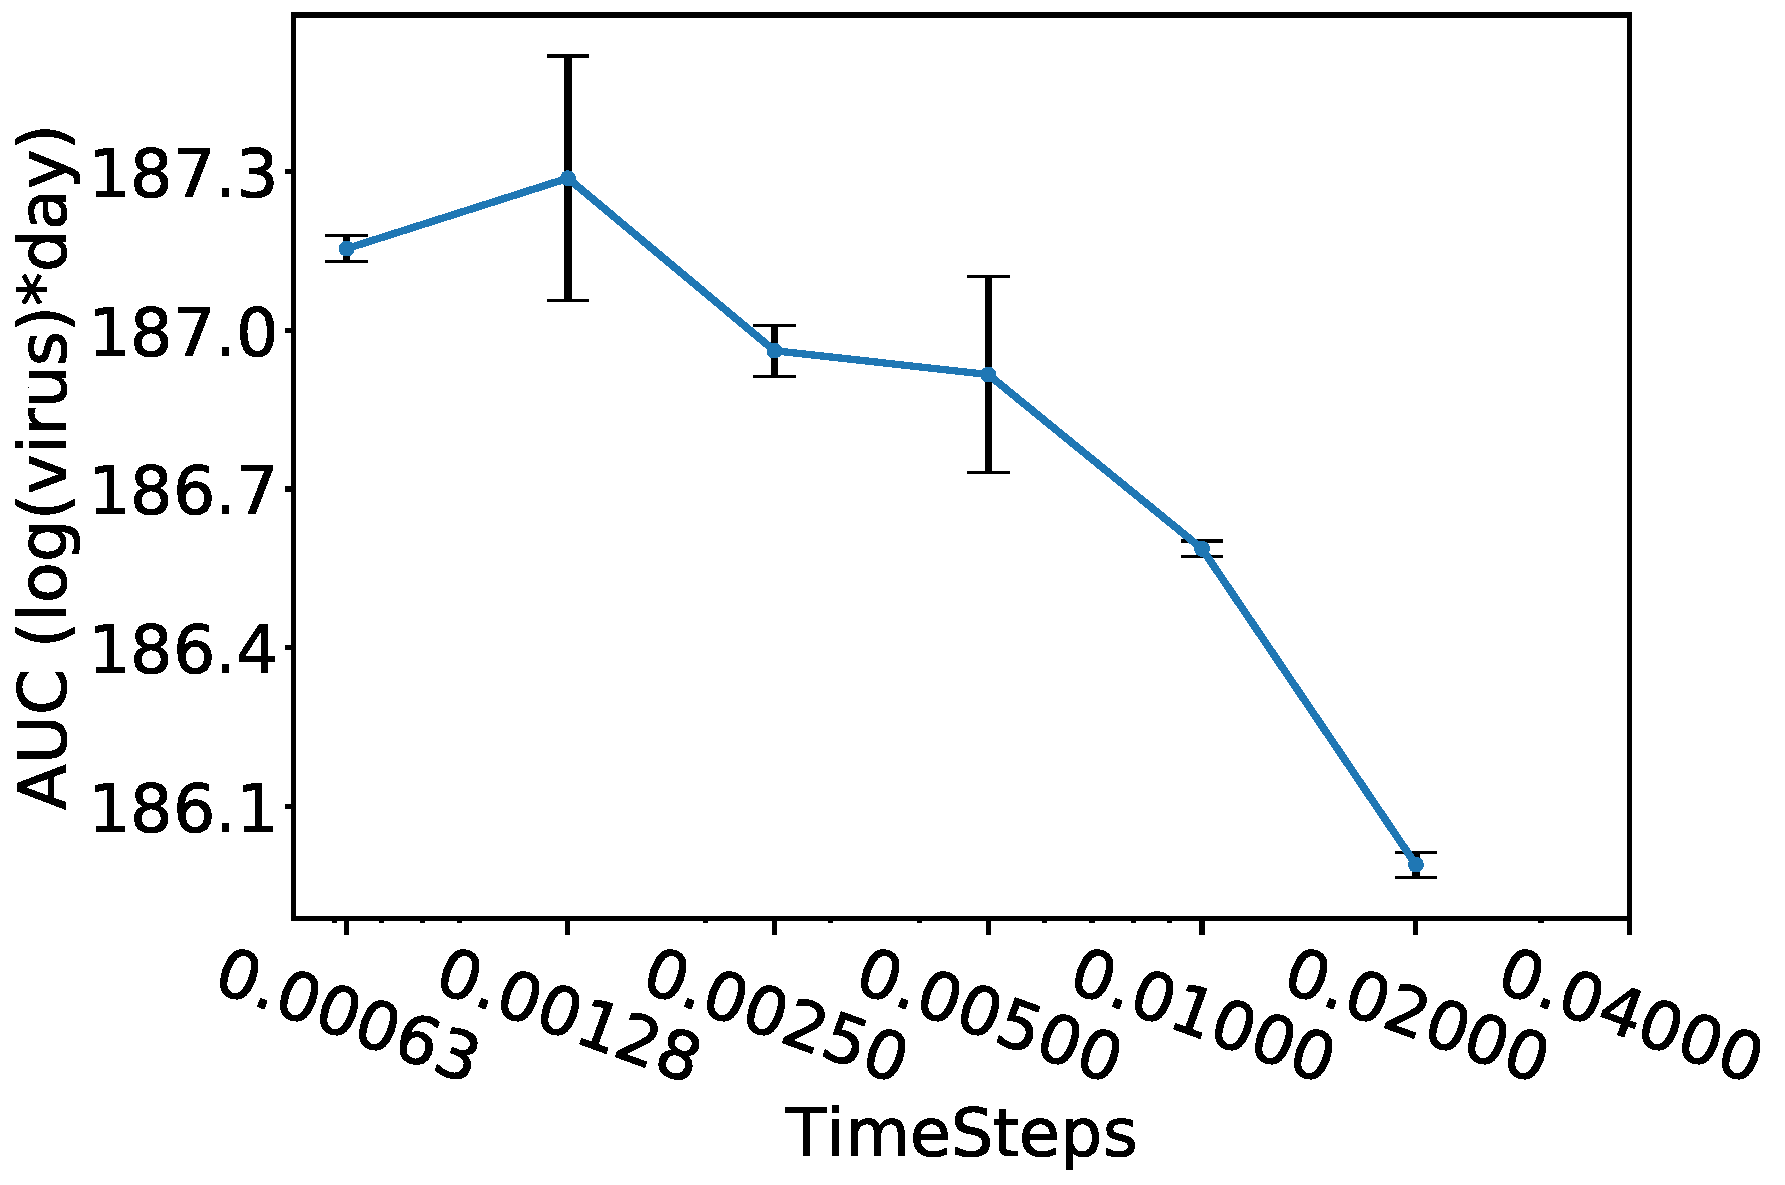
\includegraphics[width=\linewidth]{Figures/Cellfree-InitialCell-Runs_Graphs/AUC.pdf}
%        \caption{}
%        \label{fig:Peak_virus_of_both_transmission_modes}
%    \end{subfigure}
%    \begin{subfigure}[b]{0.3\linewidth}
%        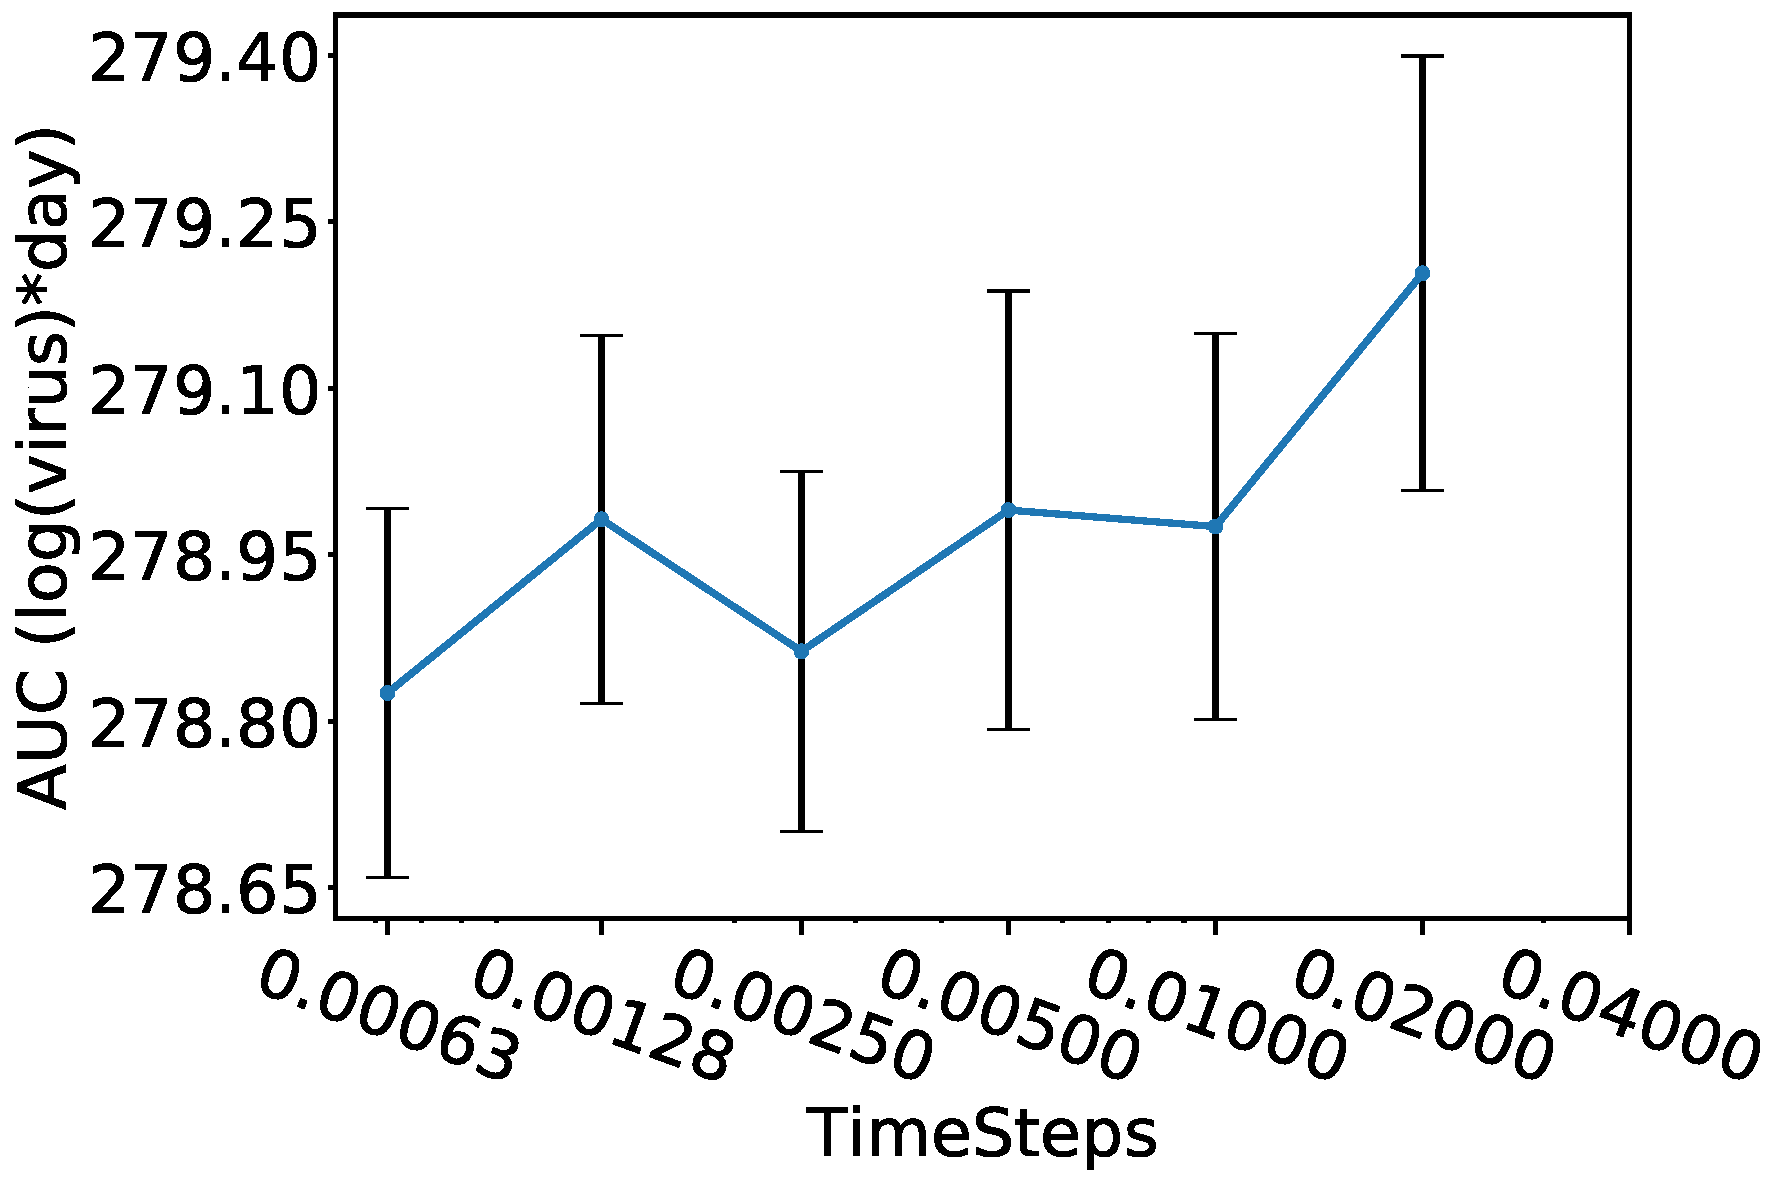
\includegraphics[width=\linewidth]{Figures/Cellfree-InitialVirus-Runs_Graphs/AUC.pdf}
%        \caption{}
%        \label{fig:Peak_virus_of_both_transmission_modes}
%    \end{subfigure}
%    \begin{subfigure}[b]{0.3\linewidth}
%        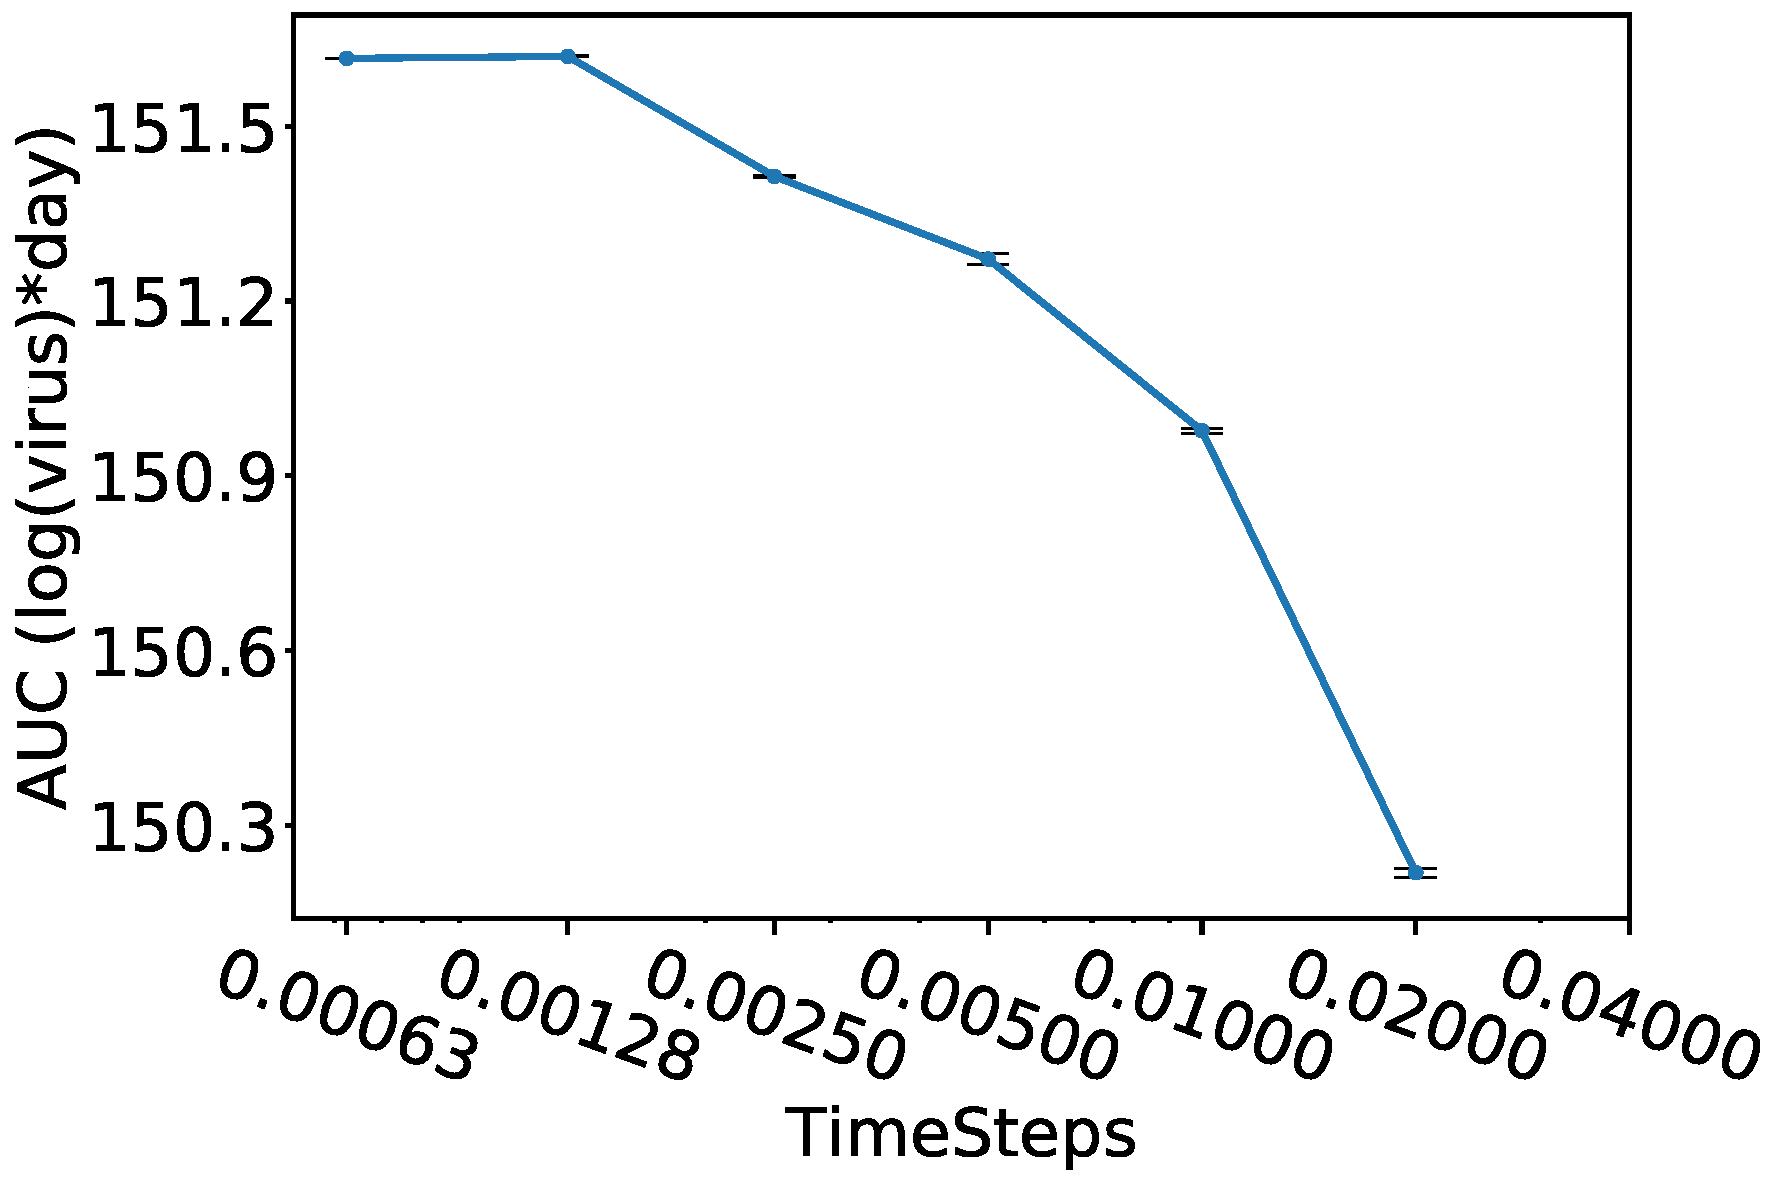
\includegraphics[width=\linewidth]{Figures/Neither-InitialVirus-Runs_Graphs/AUC.pdf}
%        \caption{}
%        \label{fig:Peak_virus_of_both_transmission_modes}
%    \end{subfigure}

%    \begin{subfigure}[b]{0.3\linewidth}
%        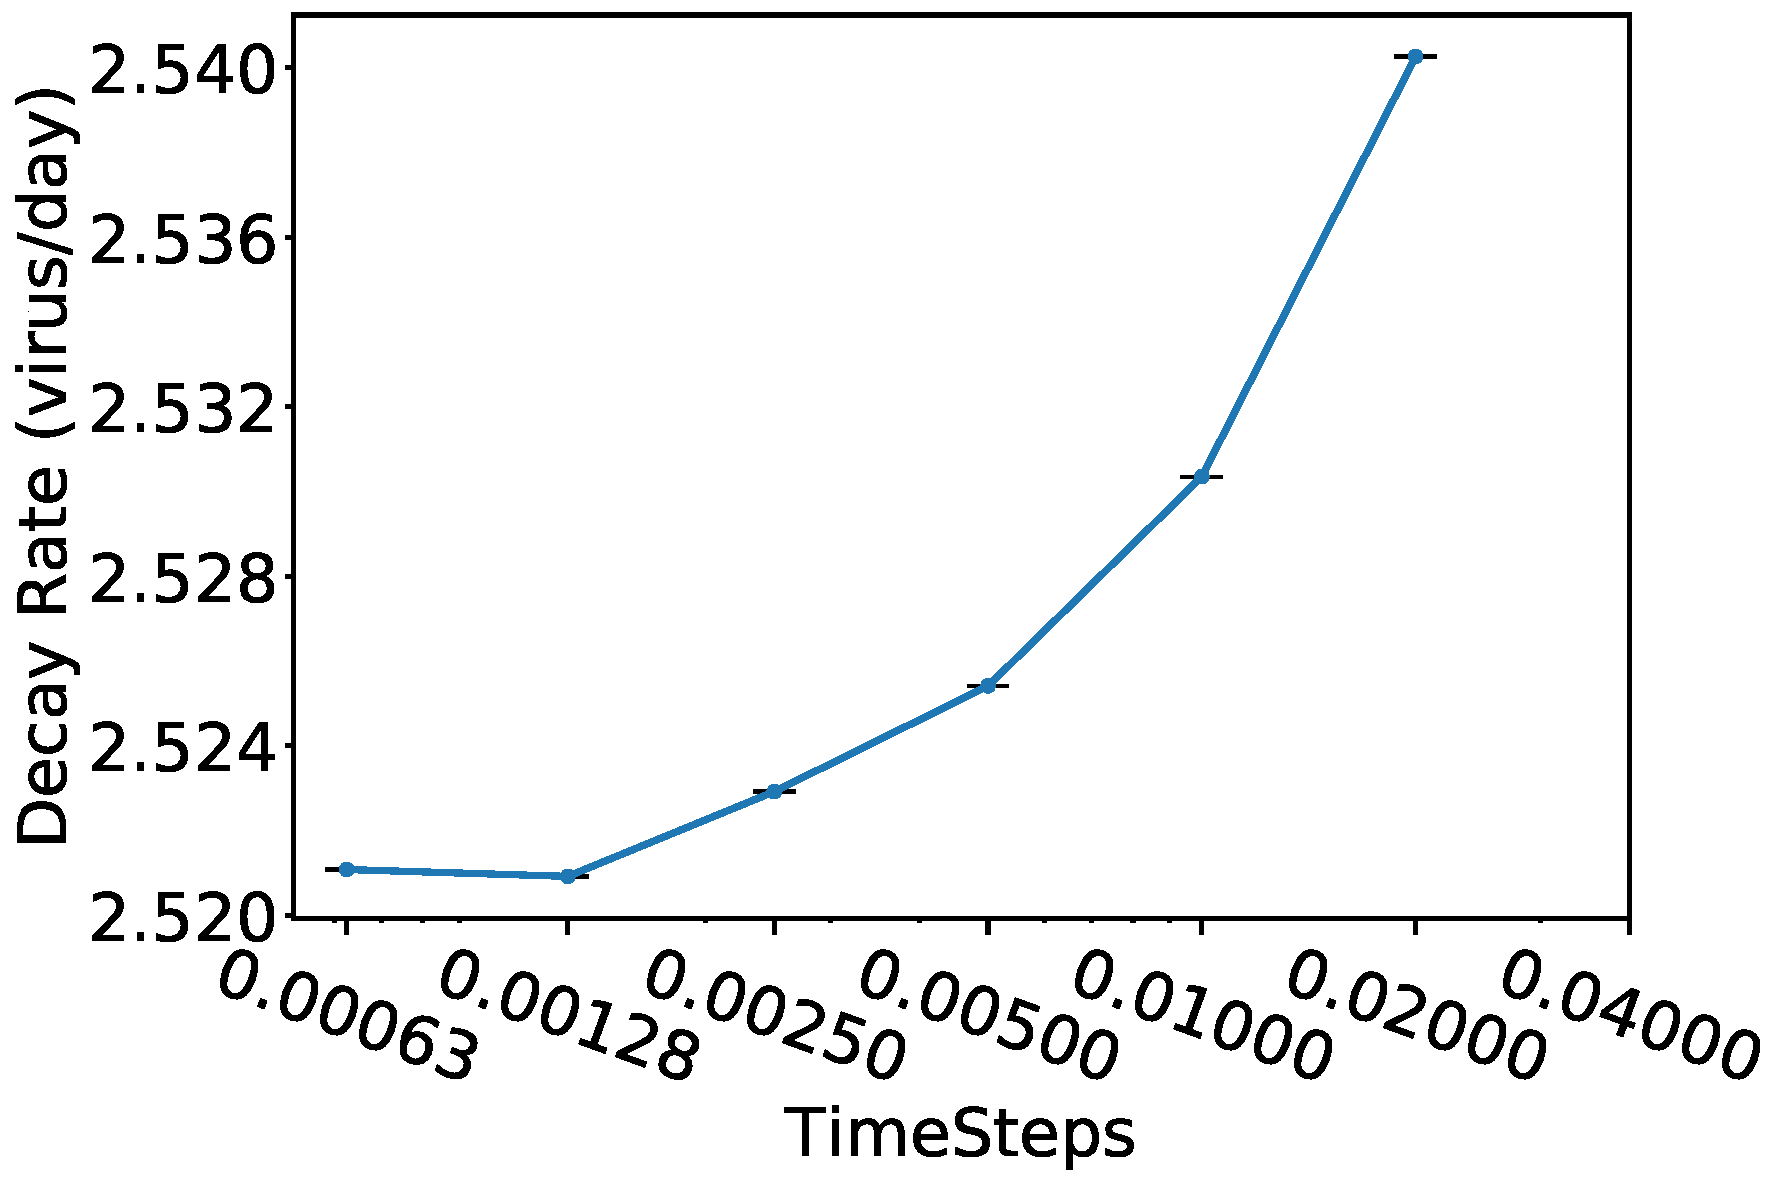
\includegraphics[width=\linewidth]{Figures/Cellfree-InitialCell-Runs_Graphs/DownSlope.pdf}
%       \caption{}
%        \label{fig:Peak_time_of_both_transmission_modes}
%    \end{subfigure}
%    \begin{subfigure}[b]{0.3\linewidth}
%        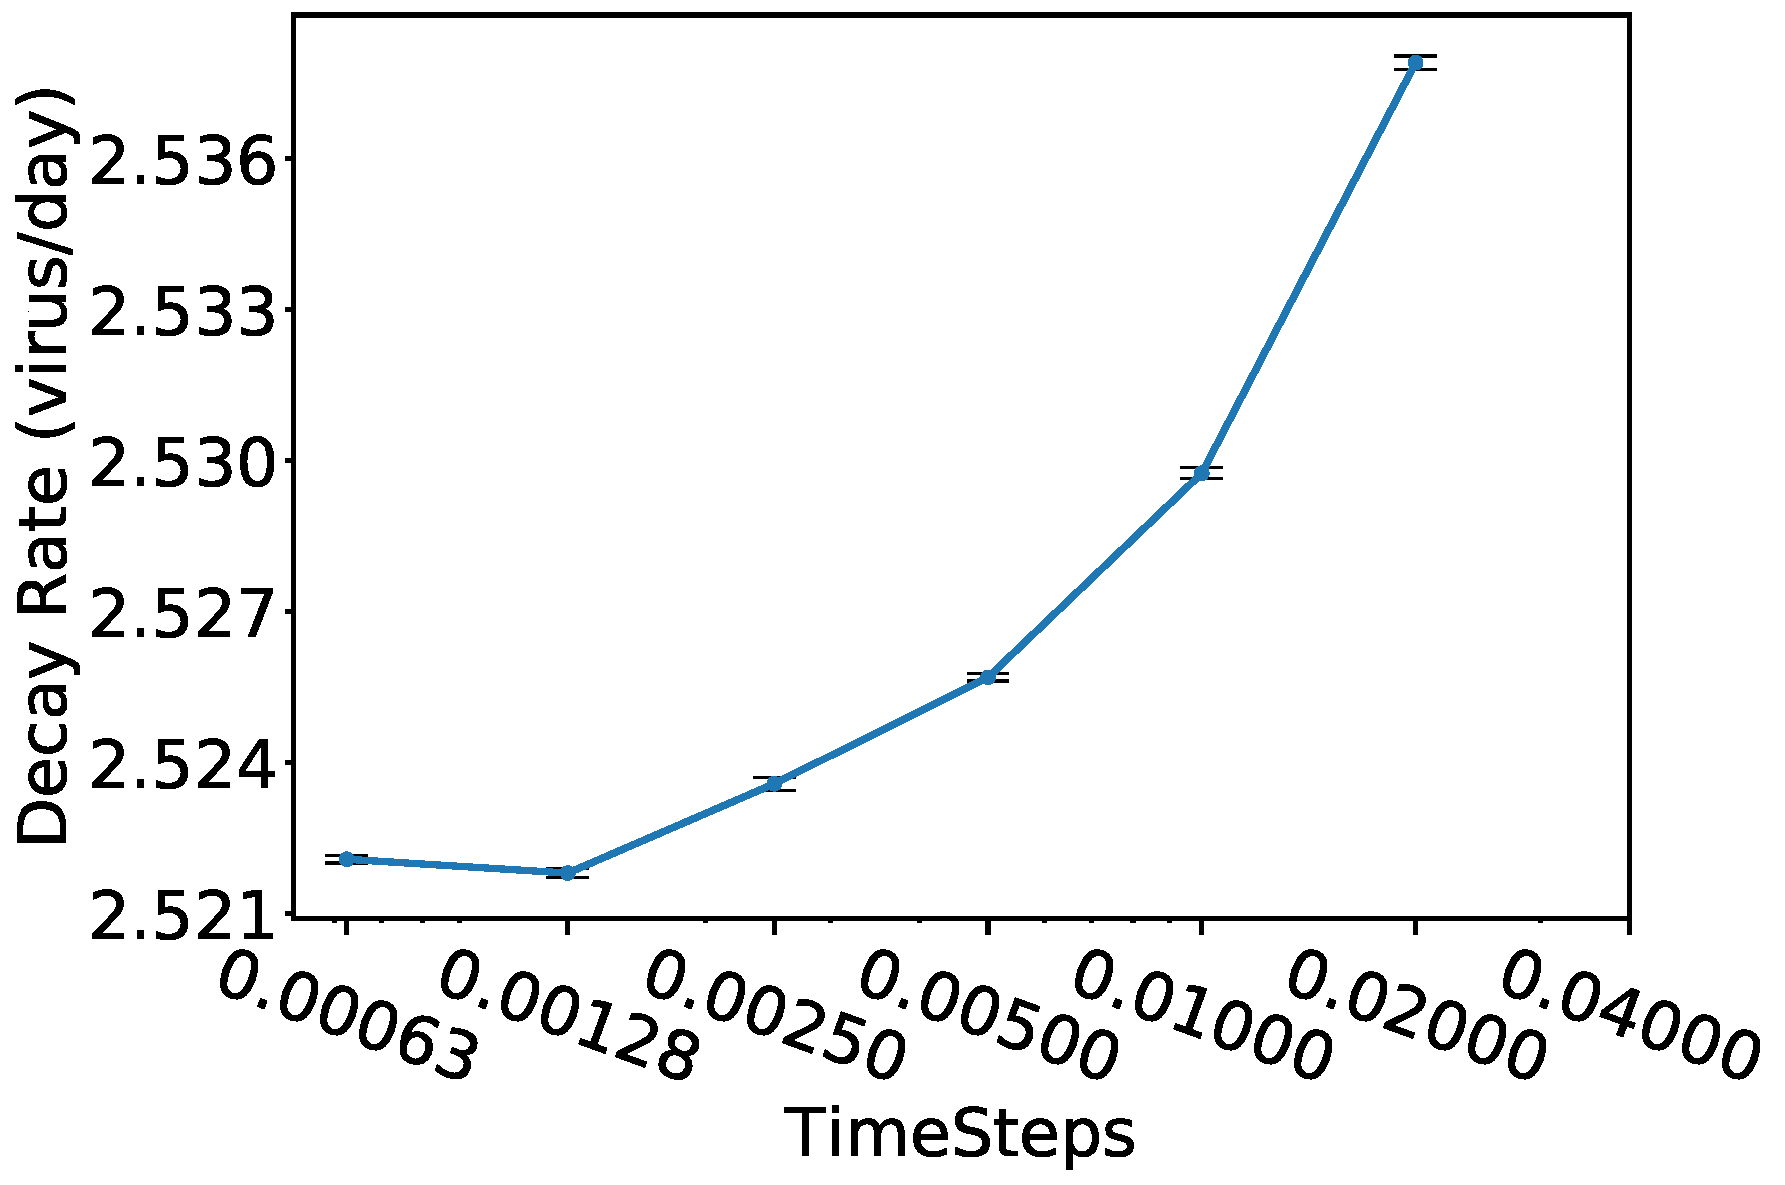
\includegraphics[width=\linewidth]{Figures/Cellfree-InitialVirus-Runs_Graphs/DownSlope.pdf}
%        \caption{}
%        \label{fig:Peak_time_of_both_transmission_modes}
%    \end{subfigure}
%    \begin{subfigure}[b]{0.3\linewidth}
%       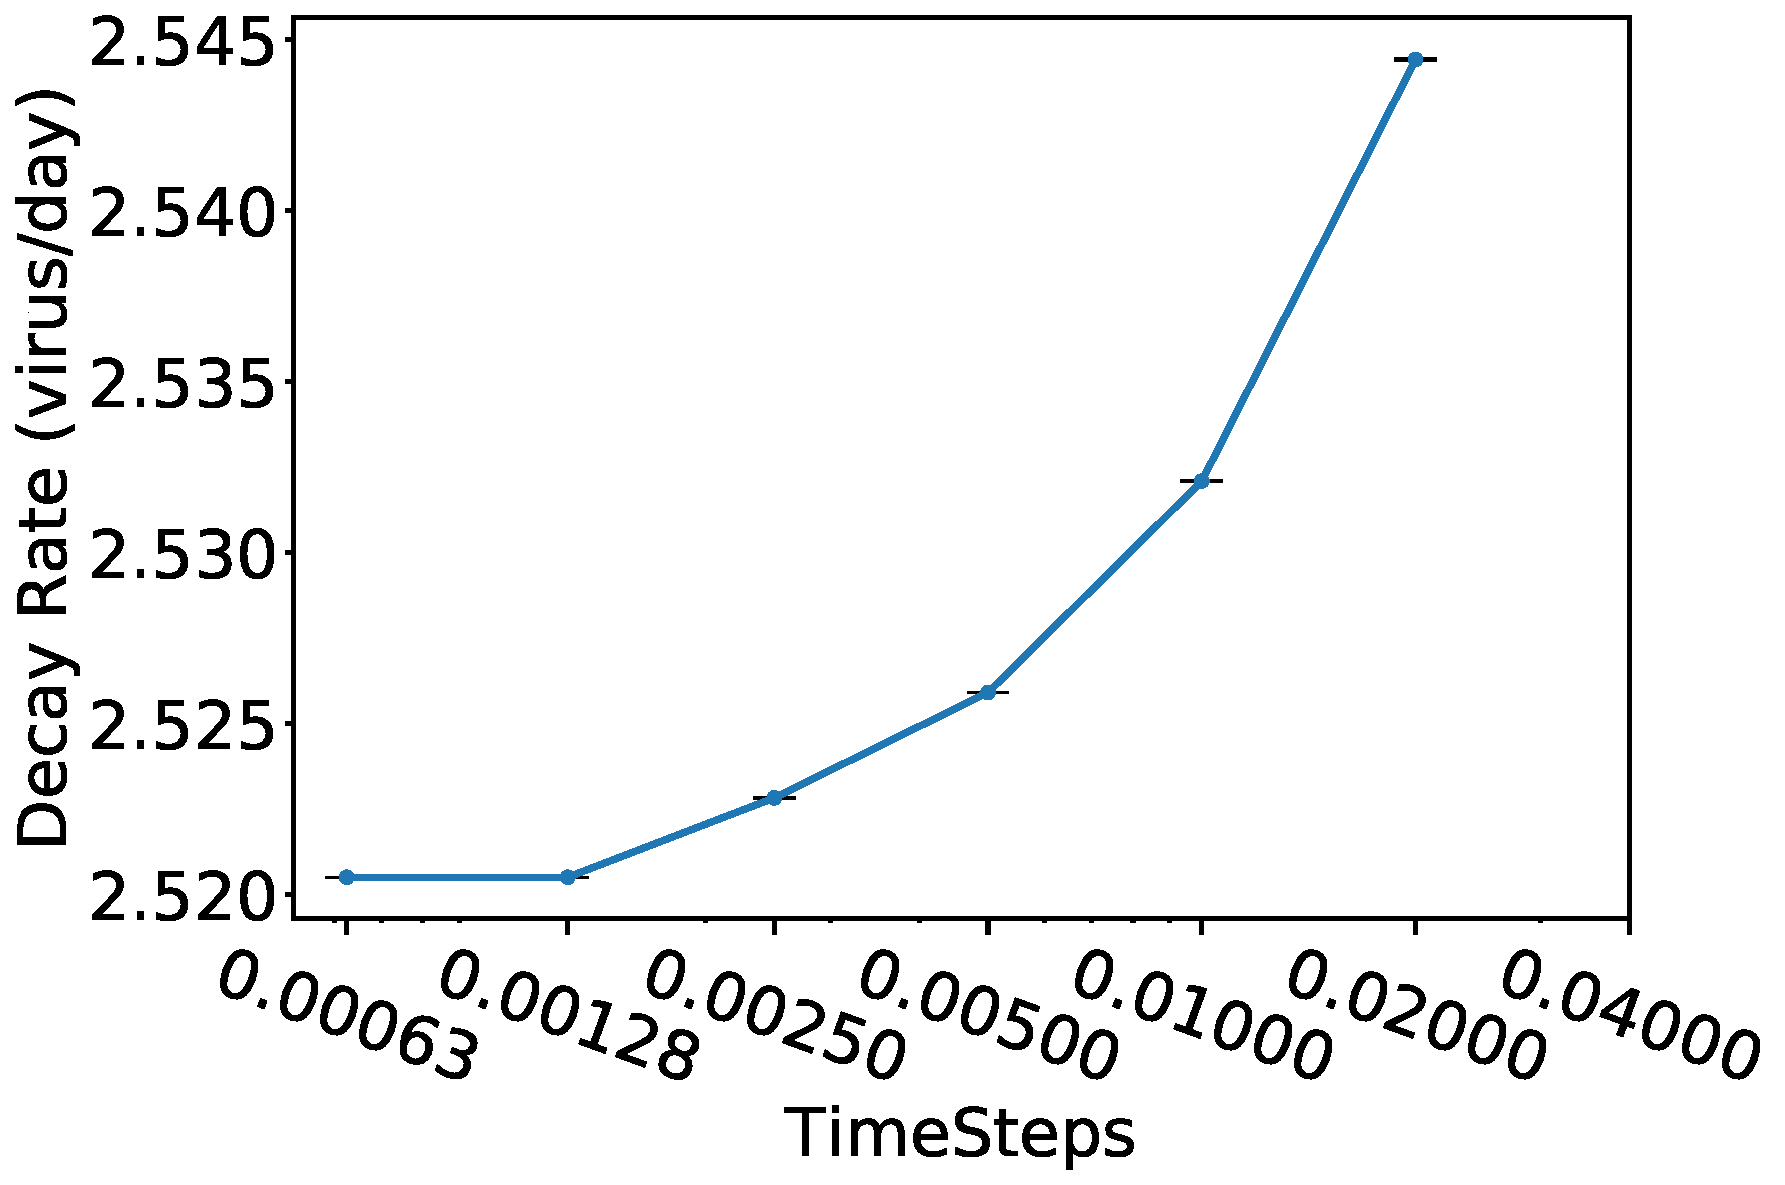
\includegraphics[width=\linewidth]{Figures/Neither-InitialVirus-Runs_Graphs/DownSlope.pdf}
%        \caption{}
%        \label{fig:Peak_time_of_both_transmission_modes}
%    \end{subfigure}

%    \begin{subfigure}[b]{0.3\linewidth}
%        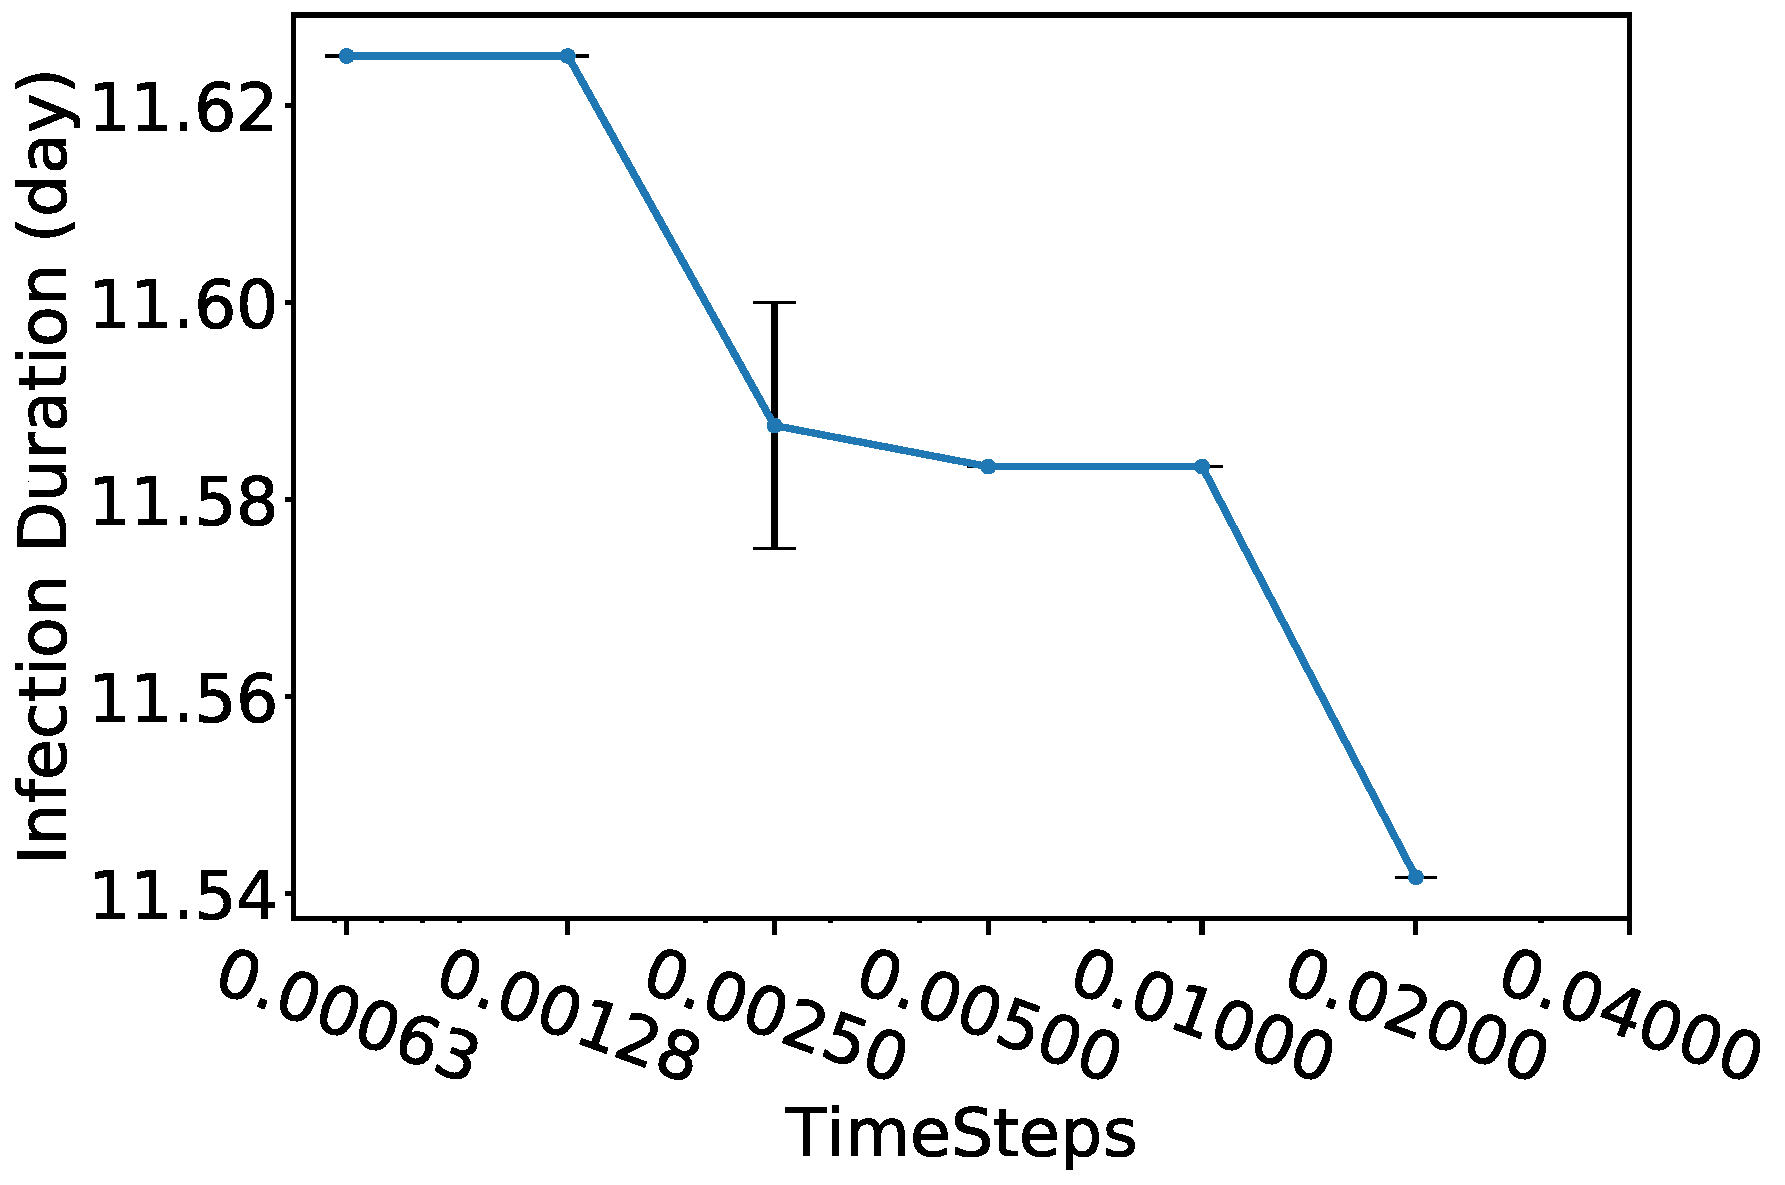
\includegraphics[width=\linewidth]{Figures/Cellfree-InitialCell-Runs_Graphs/InfectionDuration.pdf}
%       \caption{}
%        \label{fig:Growth_Rate_of_both_transmission_modes}
%    \end{subfigure}
%    \begin{subfigure}[b]{0.3\linewidth}
%        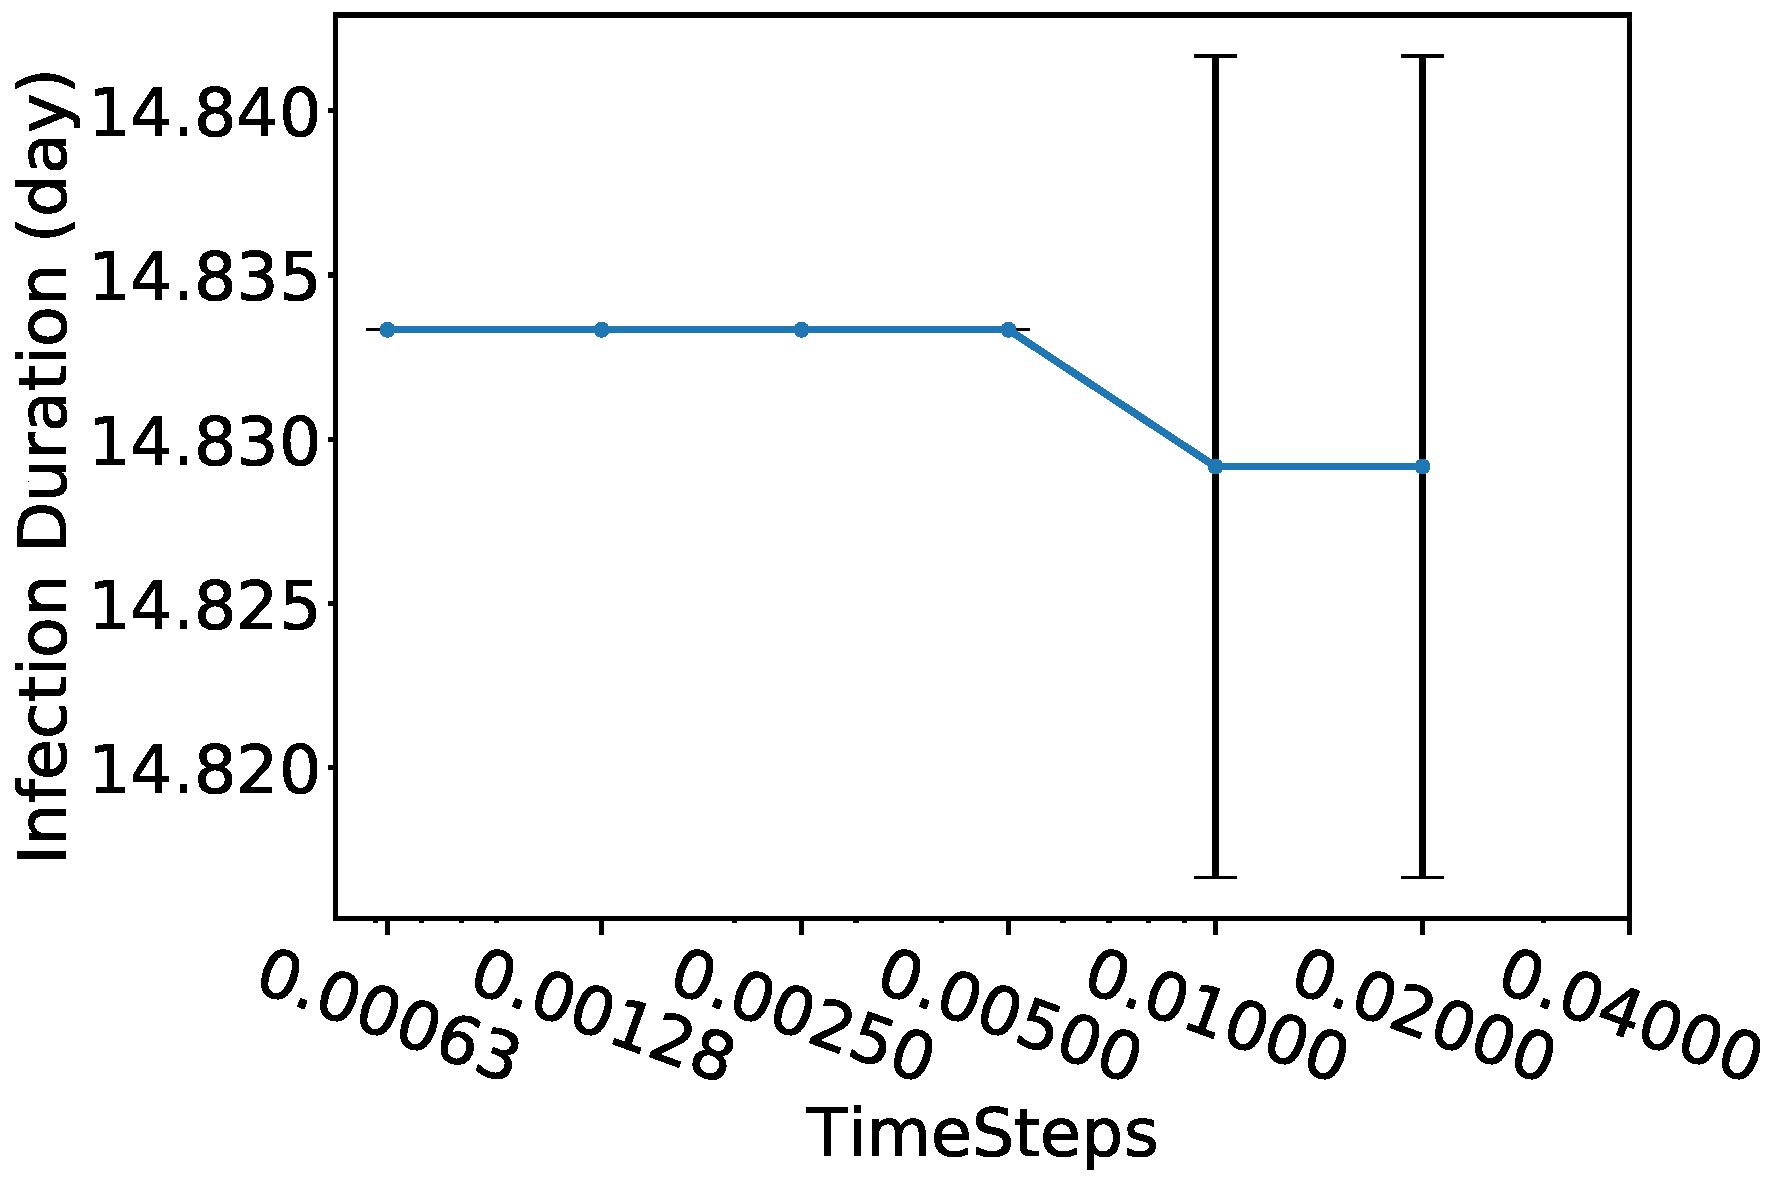
\includegraphics[width=\linewidth]{Figures/Cellfree-InitialVirus-Runs_Graphs/InfectionDuration.pdf}
%        \caption{}
%        \label{fig:Growth_Rate_of_both_transmission_modes}
%    \end{subfigure}
%    \begin{subfigure}[b]{0.3\linewidth}
%        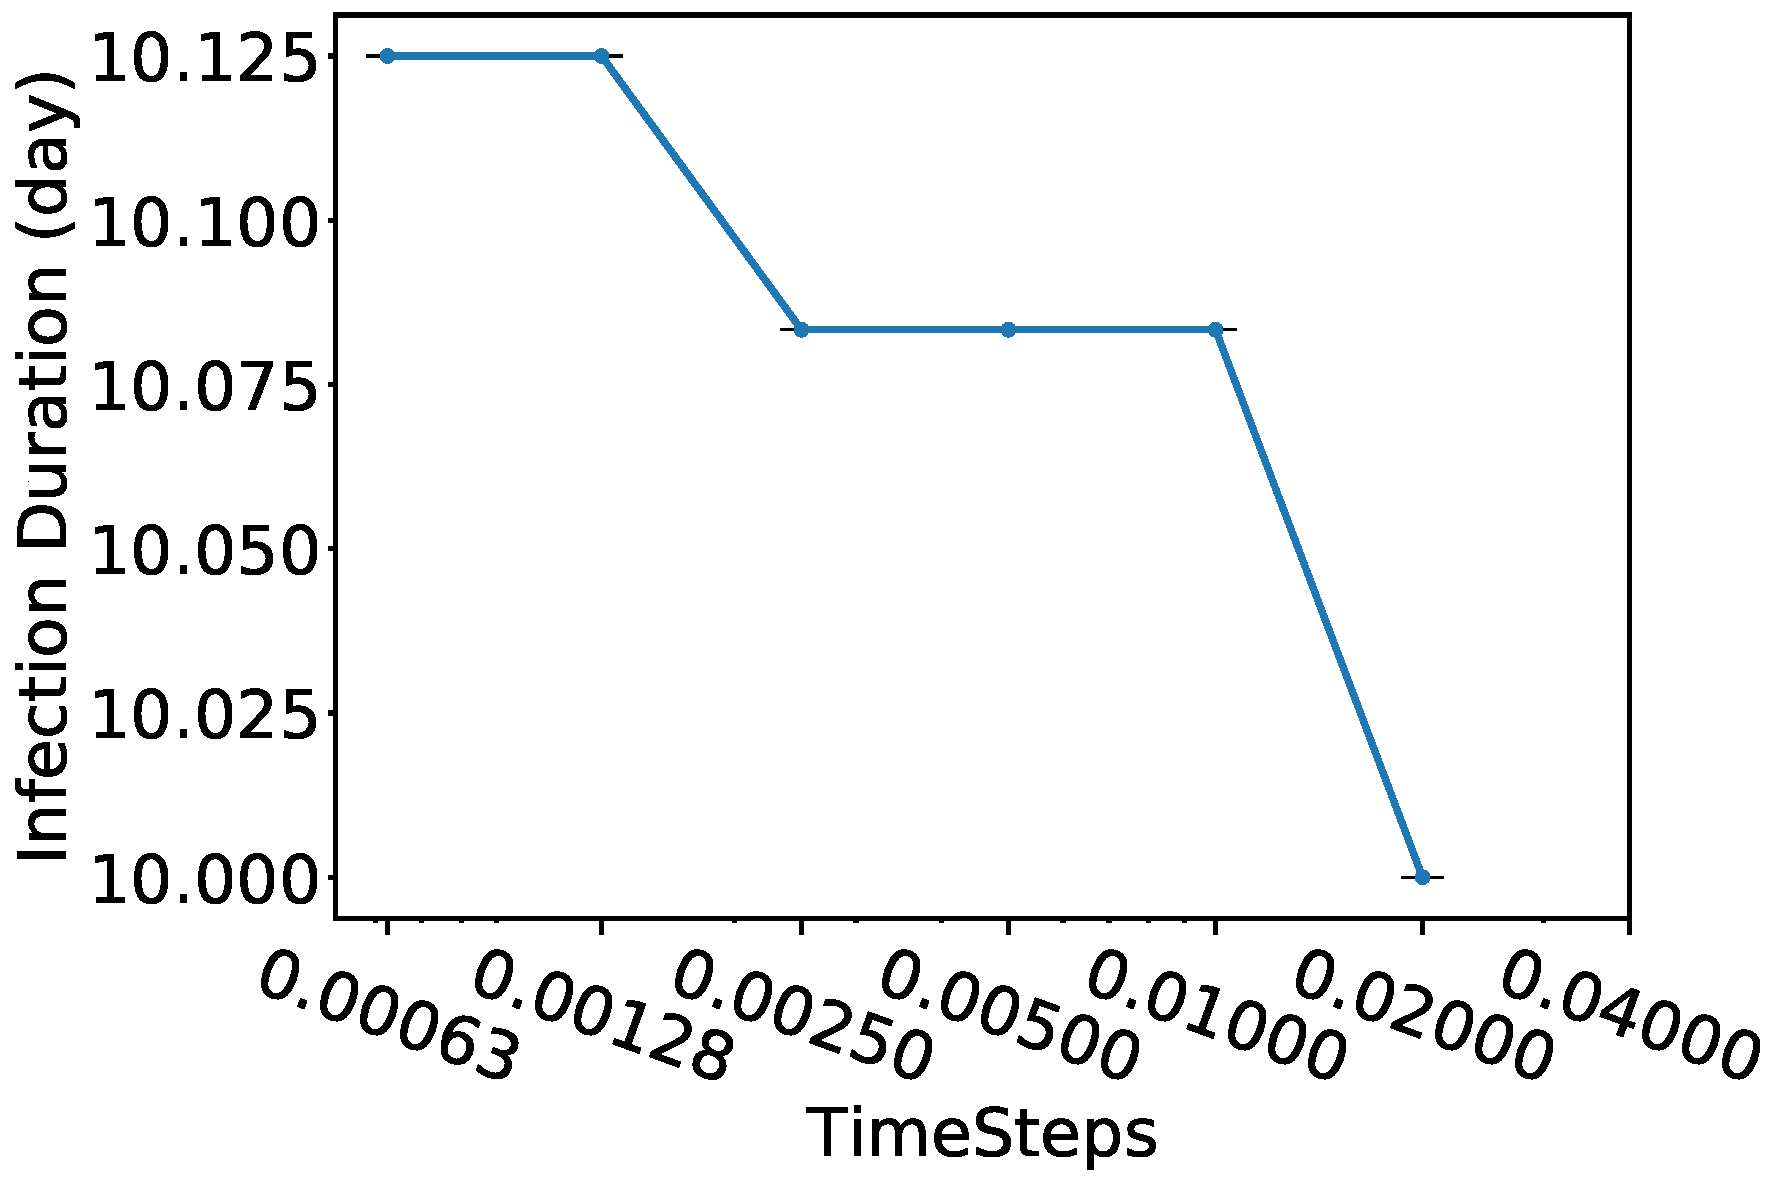
\includegraphics[width=\linewidth]{Figures/Neither-InitialVirus-Runs_Graphs/InfectionDuration.pdf}
%        \caption{}
%        \label{fig:Growth_Rate_of_both_transmission_modes}
%    \end{subfigure}

%    \begin{subfigure}[b]{0.3\linewidth}
%       \includegraphics[width=\linewidth]{Figures/Cellfree-InitialCell-Runs_Graphs/PeakViralTiter.pdf}
%        \caption{}
%        \label{fig:Decay_Rate_of_both_transmission_modes}
%    \end{subfigure}
%    \begin{subfigure}[b]{0.3\linewidth}
%       \includegraphics[width=\linewidth]{Figures/Cellfree-InitialVirus-Runs_Graphs/PeakViralTiter.pdf}
%        \caption{}
%        \label{fig:Decay_Rate_of_both_transmission_modes}
%    \end{subfigure}
%    \begin{subfigure}[b]{0.3\linewidth}
%        \includegraphics[width=\linewidth]{Figures/Neither-InitialVirus-Runs_Graphs/PeakViralTiter.pdf}
%        \caption{}
%        \label{fig:Decay_Rate_of_both_transmission_modes}
%    \end{subfigure}

%    \begin{subfigure}[b]{0.3\linewidth}
%        \includegraphics[width=\linewidth]{Figures/Cellfree-InitialCell-Runs_Graphs/TimeofPeakViralTiter.pdf}
%        \caption{}
%        \label{fig:Decay_Rate_of_both_transmission_modes}
%    \end{subfigure}
%    \begin{subfigure}[b]{0.3\linewidth}
%        \includegraphics[width=\linewidth]{Figures/Cellfree-InitialVirus-Runs_Graphs/TimeofPeakViralTiter.pdf}
%        \caption{}
%        \label{fig:Decay_Rate_of_both_transmission_modes}
%    \end{subfigure}
%    \begin{subfigure}[b]{0.3\linewidth}
%        \includegraphics[width=\linewidth]{Figures/Neither-InitialVirus-Runs_Graphs/TimeofPeakViralTiter.pdf}
%        \caption{}
%        \label{fig:Decay_Rate_of_both_transmission_modes}
%    \end{subfigure}
%    \begin{subfigure}[b]{0.3\linewidth}
%        \includegraphics[width=\linewidth]{Figures/Cellfree-InitialCell-Runs_Graphs/UpSlope.pdf}
%        \caption{}
%        \label{fig:Decay_Rate_of_both_transmission_modes}
%    \end{subfigure}
%    \begin{subfigure}[b]{0.3\linewidth}
%        \includegraphics[width=\linewidth]{Figures/Cellfree-InitialVirus-Runs_Graphs/UpSlope.pdf}
%        \caption{}
%        \label{fig:Decay_Rate_of_both_transmission_modes}
%    \end{subfigure}
%    \begin{subfigure}[b]{0.3\linewidth}
%        \includegraphics[width=\linewidth]{Figures/Neither-InitialVirus-Runs_Graphs/UpSlope.pdf}
%        \caption{}
%        \label{fig:Decay_Rate_of_both_transmission_modes}
%    \end{subfigure}
    \caption{Characteristics of the viral titer curves where measured for each of the seven time steps and the different scenerios.\label{fig_AspectGraphs}}
\end{minipage}
\end{figure}

\subsection{Fitting the model to data}

We fit the model to experimental \emph{in vitro} data \citep{pinilla12} via minimization of the SSR. The initial condition of the simulations were: 501535 cells in the dish (similar to the number of cells in a typical 24-well plate \citep{Number_of_cells_in_a_dish_noauthor_useful_nodate}), 50 initial infected cells, and no virus in the dish. In figure \ref{fig_DataFit}, the median curve of ten simulations, using the best fit parameters, is plotted in dark blue alongside the data in green. Our best fit parameters are presented in Table \ref{tab_datafit_params}. Although the same data was used, some of our parameter estimates differ from those reported in Pinilla et al.\ \citep{pinilla12}. Our best fit $\tau_I$ is smaller than the $\tau_I = \SI{49}{\hour}$ reported by Pinilla et al., while our best fit $\tau_E$ is larger than the $\tau_E = \SI{6.6}{\hour}$ found by Pinilla et al., and the best fit $c$ is larger than $c = \SI{0.13}{\per\hour}$. Some of this discrepancy might be due to the inclusion of spatial effects in the ABM, but Pinilla et al.\ also used more data --- they used both a single cycle and multiple cycle experiment as well as viral RNA measurements --- to constrain the parameter estimates. All in all, the ABM/PDEM model can replicate the viral titer measurements of a typical infection via fitting where the fitting process uses standard packaged fitting algorithms and the computational time for fitting is less than 24 hours from inital guess to best fit.

\begin{table}
\centering
\caption{Best fit parameter values from fitting model to experimental data \citep{pinilla12}. \label{tab_datafit_params}}
\begin{tabular}{llc}
\hline
Parameter & Meaning & Value \\
\hline
$\beta$ & Infection rate & 54 $/\mathrm{h}$ \\
$p$ & Viral production rate & 3000 $/\mathrm{h}$ \\
$c$ & Viral clearance rate & 0.25 $/\mathrm{h}$ \\
$D$ & Diffusion coefficient & 2.2$\times 10^{-8}$ $\mathrm{m}^2/\mathrm{h}$ (fixed) \\
$\tau_E$ & Mean eclipse duration & 16 $\mathrm{h}$ \\
$\eta_E$ & Eclipse shape parameter & 30 (fixed) \\
$\tau_I$ & Mean infectious lifespan & 26 $\mathrm{h}$ \\
$\eta_I$ & Infectious shape parameter & 100 (fixed) \\
\end{tabular}
\end{table}

\begin{figure}
\centering
    \includegraphics[width=0.6\linewidth]{Figures/DataFit.pdf}
\caption{The ten simulated titer curves and corresponding median curve are plotted in blue. The experimental cell-free transmission data \citep{pinilla12} is plotted in green. The median curve has the minimal SSR with respect to the experimental data, when using the best fit parameters. The best fit parameters are shown in \ref{tab_datafit_params}. \label{fig_DataFit}}
\end{figure}

\section{Summary}

In this paper, we describe the construction of a hybrid ABM/PDEM model to investigate spatially extended viral infections. While the formulation of the model is similar to other ABM/PDEM models of viral spread \citep{beauchemin_simple_2005, bauer_agent-based_2009}, we have implemented our model to run on GPUs, vastly improving the simulation speed of these models. This allows for efficient replication of \emph{in vitro} infections with a realistic number of cells. This will help lead to a better understanding of virus-cell dynamics \emph{in vitro} \citep{blahut21}, but could also help realize the goal of simulating infections \emph{in vivo} \citep{laubenbacher21}. The faster simulations also allowed us to use standard ODE model-fitting techniques to fit this model to experimental data, making it possible to quickly parameterize these models to reproduce dynamics of different viruses. Previously, researchers have had to develop other techniques to help speed up fitting of ABMs to experimental data, including reducing the sampled parameter space \citep{li17}, and mapping of ABM outputs to simpler functions \citep{tong_development_2015, read16}. These techniques coupled with simulation of ABMs on GPUs could potentially allow for real-time parameter estimation of models for use in patient care. This is particularly useful for a novel pandemic virus that can be simulated such that trial runs of test drugs can be performed and viral infection severity for a patient can potentially be predicted.

